\documentclass[10pt]{article}
\usepackage[verbose, a4paper, hmargin=2.5cm, vmargin=2.5cm]{geometry}

\usepackage{fontspec}
\usepackage{ctex}
\usepackage{paratype}

\usepackage{amsmath}
\usepackage{amssymb}
\usepackage{amsfonts}
\usepackage{esint}
\usepackage{stmaryrd}


\setmainfont{Times New Roman}

\setsansfont{Arial}
\setmonofont{Courier New}

\usepackage{makecell}
\usepackage{wasysym}
\usepackage{pifont}
\usepackage[export]{adjustbox}
\usepackage{graphicx}
\usepackage{mdframed}
\usepackage{booktabs,array,multirow}
\usepackage{tabularx}
\usepackage{hyperref}
\usepackage{enumitem}
\usepackage{caption}
\usepackage{makecell}
\hypersetup{colorlinks=true, linkcolor=blue, filecolor=magenta, urlcolor=cyan,}
\urlstyle{same}
\usepackage[most]{tcolorbox}
\definecolor{mygray}{RGB}{240,240,240}
\tcbset{
  colback=mygray,
  boxrule=0pt,
}
\graphicspath{ {./images/} }
\newcommand{\HRule}{\begin{center}\rule{0.9\linewidth}{0.2mm}\end{center}}
\newcommand{\customfootnote}[1]{
  \let\thefootnote\relax\footnotetext{#1}
}
\newcommand{\lt}{\mathrel{<}}
\newcommand{\gt}{\mathrel{>}}
\newcommand*\circled[1]{\tikz[baseline=(char.base)]{\node[shape=circle,draw,inner sep=1.5pt] (char) {\small #1};}}
\setcounter{MaxMatrixCols}{256}
\begin{document}
\title{运动规划中的混合整数规划}
\author{Daniel Ioan\thanks{通讯作者. 电子邮箱: daniel.ioan@l2s.centralesupelec.fr. 法国巴黎南大学-中央苏佩雷克-国家科学研究中心信号与系统实验室，巴黎萨克雷大学} \and Ionela Prodan\thanks{电子邮箱: ionela.prodan@lcis.grenoble-inp.fr. 格勒诺布尔阿尔卑斯大学，格勒诺布尔工程学院(Université Grenoble Alpes)，LCIS，F-26000，瓦伦西亚，法国} \and Sorin Olaru\thanks{电子邮箱: sorin.olaru@l2s.centralesupelec.fr. 法国巴黎南大学-中央苏佩雷克-国家科学研究中心信号与系统实验室，巴黎萨克雷大学} \and Florin Stoican\thanks{电子邮箱: florin.stoican@upb.ro. 罗马尼亚UPB自动控制与系统工程系} \and Silviu-Iulian Niculescu\thanks{电子邮箱: silviu.niculescu@l2s.centralesupelec.fr. 法国巴黎南大学-中央苏佩雷克-国家科学研究中心信号与系统实验室，巴黎萨克雷大学}}
\date{}
\maketitle

\section*{文章信息}

关键词:MIP(混合整数规划)，运动规划，MPC(模型预测控制)，路径跟踪，轨迹跟踪，任务分配，碰撞避免

\section*{摘要}

本文回顾了使用MIP(混合整数规划)在运动规划领域的过去和现在的研究成果与方法.尽管在2000年代初，MIP仍被视为解决运动规划相关问题的犹豫方法，但如今，随着计算能力的提升和理论的进步，其广泛的建模能力和多功能性逐渐凸显，应用和认可度不断提高.这类控制问题本质上涉及从有限备选方案中选择，或在非凸域上进行约束优化.在这两种情况下，MIP已被证明是一种高效的建模技术，本文将对此进行说明.此外，重点还放在现有的实现方案和文献中记录的各种实验验证上.

\section{引言}

本节介绍一些实际中的一般性问题/情境，这些问题实际上归结为包含整数和实数变量的优化问题，可以类比为开环或闭环控制问题.同时，为了更广泛的视角，还介绍了通过MIP方法解决的问题类别.

\subsection{动机与背景}

在超过60年的发展历程中，整数规划领域因其出色的建模能力和灵活性而在数学界得到了广泛研究.近年来(主要是过去二十年)，主要由于计算能力的提升，整数规划引起了控制和机器人领域的关注.存在大量可以通过MIP框架/方法处理的决策问题.

MIP(混合整数规划)是一种数学优化问题，其中部分或全部变量为整数.

正如其名称所示，MIP(混合整数规划)代表一种数学优化问题，其目标是最小化或最大化线性、二次函数或有时更一般的准则，约束条件为线性(或非线性)等式(或不等式)，并存在一些(非空)整数和实数变量子集作为参数(Jünger等，2009；Williams，2013).

MIP被用来建模多个设计问题和决策过程.

从更广泛的角度来看，MIP用于建模多个设计问题和决策过程.以典型的物流问题为例:一个每天平均处理50个航班的机场.该机场只有四条跑道.出现的任务分配问题是将航班分配到跑道上，以实现跑道的高效和均匀使用，同时遵守一些规定(例如，两次连续降落/起飞之间的时间间隔，或同时起飞的两条跑道之间的最小距离).另一个经典情境是著名的旅行商问题及其变体，旅行商希望在最短时间内拜访若干客户或覆盖最短距离.这在多个领域都有应用(例如，燃气轮机引擎的检修或X射线晶体学 Matai、Singh和Mittal，2010).上述问题可以凭直觉、经验或试错法解决，但在关键情况下，为了认证，必须进行精确的数学建模.当然，还有许多其他应用场景也可能采用MIP.例如，能源传输网络中的最优潮流Bahiense、Oliveira、Pereira和Granville(2001)，或在复杂环境中的运输问题.考虑在峡湾区域内移动的船只，为了安全到达目的地，船只应沿给定路径行驶并避免与峡湾碰撞.因此，可行区域是非凸的，必须高效描述.



以下简要介绍通过MIP建模的问题类型分类.第一类问题涉及整数数量(即离散/量化的输入或输出)，例如背包问题(Williams，2013).对于这类问题，MIP似乎不是最自然的首选，但通常比传统方法(例如使用经典线性规划并将解近似到最接近的整数值)更优.

另一类可用MIP模型化的问题是涉及逻辑条件的问题，详见:Bemporad和Morari(1999)、Williams(2013)、Smith和Taskin(2008).例如，在Bemporad和Morari(1999)中，采用Williams(2013)中的符号，将布尔代数工具整合，允许将连续变量上的逻辑条件转化为混合整数不等式(涉及连续和二元变量的线性不等式).

此外，MIP也是序列和/或分配问题(也称组合问题)(Smith \& Taskin，2008)的常用建模工具，包括典型的任务分配问题及其变体(如旅行商问题，Dantzig、Fulkerson和Johnson(1954)).这类问题可以很容易扩展到网络(图论)问题:在PERT(项目评估与审查技术)网络上的资源分配(Williams，2013).

最后，但对本文目的最为重要的是，MIP被证明是一种引人入胜的非线性(Bemporad \& Morari，1999；Vielma，2015)和/或非凸性(Prodan、Stoican、Olaru和Niculescu，2015；Richards \& How，2005)建模方法.许多控制工程问题本质上具有非线性和/或非凸性.因此，随着对基于优化的控制的兴趣日益增加(Mayne、Rawlings、Rao和Scokaert，2000)，MIP已成为一种关键技术，能够在优化问题中包含逻辑决策和非凸约束.因此，MIP在控制中的应用可以体现在:分段线性系统识别(Bemporad、Roll和Ljung，2001；Roll、Bemporad和Ljung，2004)、分配问题(Alighanbari、Kuwata和How，2003)、持续激励控制(Mar-afioti、Stoican、Bitmead和Hovd，2012)、混合系统控制(Bemporad \& Morari，1999)、故障检测(Stoican、Olaru、Seron和De Doná，2012)或运动规划(Prodan等，2015；Richards \& How，2002).正如标题所示，在本综述中，主要目标是识别并总结基于MIP的运动规划的最新研究进展.因此，接下来我们对其他使用MIP的控制领域关注较少，即使在全文中偶尔会提及相关文献，供感兴趣的读者参考其他MIP控制主题的资料.

\subsection{贡献}

本文对多智能体运动规划领域中基于混合整数框架的突破性研究成果和未解问题进行了详细的文献综述.本工作可为控制和优化研究界提供帮助，帮助快速识别该领域的既有、及时且相关的研究主题，同时也缩短文献回顾的时间，尽管我们承认本次综述并非详尽无遗，而仅涵盖了作者在过去十年中在这些主题上的经验.

据作者所知，尚无其他关于该主题的详尽综述，尽管文献中存在一些具有不同目标的有价值的尝试.例如，Richards和How(2005)在教程中简要介绍了如何将MIP应用于(反馈)控制.此外，Smith和Taskin(2008)的论文提供了对MIP建模的简明介绍，涵盖了MIP公式的基本概念(原则和一些实用技巧)，同时讨论了广泛用于解决MIP问题的技术.此外，Jünger等(2009)出版的《50年整数规划:从早期到最先进》提供了整数规划领域的历史视角，讨论了MIP在理论、算法和计算方面的五十余年发展.此外，还有一些具有重要影响的综述，例如Vielma(2015)，回顾了先进的MIP公式技术，旨在为某类决策问题提供更强或更紧凑的公式.这些工作要么局限于编程方面，要么关注决策制定或狭窄的控制设计主题.因此，我们决定将综述重点放在基于MIP的控制问题，特别是源自运动规划这一活跃研究领域的应用，该领域在汽车、机器人或多智能体系统等方面具有广泛应用，仅举几例.

\subsection{大纲}

本文其余部分的组织结构如下.第2节简要介绍了MIP数学描述的演变，提供了这些公式所需的基本前提.第3节展示并详细说明了运动规划中的标准基于MIP的问题，介绍了此类问题中采用的通用控制策略.接着，第4节过渡到多智能体系统及涉及MIP的编队控制问题.第5节简要概述了在基于MIP的导航问题中采用的控制架构.此外，第6节简要介绍了文献中MIP解决方案的软件和硬件实现.第7节简要介绍了MIP的运动规划替代方案.最后，我们总结了MIP基础运动规划的结论、面临的挑战以及未来研究的建议.

\subsection{符号}

在本文中，我们使用以下标准符号.逻辑运算符: \(\land\) (与)， \(\vee\) (或)和 \(\neg\) (否定).两个集合的Minkowski和: \(A \oplus  B = \{ x : x = a + b,a \in  A,b \in  B\}\) .对于 \(x \in  {\mathbb{R}}^{d}\) ，我们用 \(\parallel x{\parallel }_{Q}^{2} = {x}^{\top }{Qx}\) 表示.给定紧集 \(S \subset  {\mathbb{R}}^{n},{\mathcal{C}}_{X}\left( S\right)\) ，表示 \(S\) 在 \(X\) 上的补集，而 \({cl}\left( S\right)\) 是子集 \(S\) 的闭包.对于任何多面体 \(P \subset  {\mathbb{R}}^{d},\mathcal{V}\left( P\right)\) ，其顶点组成的集合为(有限)集合.任何多面体(即有界多面体)都可以用半空间的交或极点的凸包表示: \(P = \left\{  {x : {s}_{i}^{\top }x \leq  {r}_{i}}\right.\) ， \(\forall i\}  = \left\{  {x : x = \sum {\alpha }_{j}{v}_{j},\sum {\alpha }_{j} = 1,{\alpha }_{j} \geq  0,\forall j}\right\}\) .对于离散集 \(\mathcal{I},\# \mathcal{I}\) ，表示其基数.

\section{MIP 公式}

存在多种MIP公式，可以追溯到20世纪80年代早期(甚至更早)，每种都强调MIP的建模能力.这些公式具有共同的特征:用二进制和/或整数变量编码离散决策.这些决策出现在不同的问题中，每个问题使用特定的公式.本节简要介绍最常用的MIP技术，并同时引入一些基本的理论概念和工具.

虽然广义析取规划(GDP)未在运动规划中明确使用，但我们简要介绍它，以体现通过MIP进行析取建模的普遍性.

\subsection{广义析取规划}

广义析取规划(GDP)首次出现在Raman和Grossmann(1994)中，旨在利用定量和定性信息以最优方式解决化工问题.为此，定性信息通过析取和逻辑命题表示.与MIP相比，GDP方法具有相对更紧凑的公式，因为逻辑条件不是通过布尔代数和不等式转换，而是以其自然(逻辑)形式表示.换句话说，GDP将代数和逻辑方程的结合表示为如下典型GDP(1):

\begin{subequations}
  \begin{gather}
    \mathop{\min }\limits_{x}f\left( x\right)  + \mathop{\sum }\limits_{k}{c}_{k} \\
    \text{ s.t. }r\left( x\right)  \leq  0,x \in  {\mathbb{R}}^{n},\;{c}_{k} \in  \mathbb{R}\text{ , } \\
    \mathop{\bigvee }\limits_{{j \in  {J}_{k}}}\left\lbrack  \begin{matrix} {Y}_{jk} \\  {g}_{jk}\left( x\right)  \leq  0 \\  {c}_{k} = {\gamma }_{jk} \end{matrix}\right\rbrack  ,\;k \in  K,\\
    \Omega \left( Y\right)  = \text{ true, }\;{Y}_{jk} \in  \{ \text{ true, false }\} ,\\
  \end{gather}
\end{subequations}


其中 \(r\left( x\right)\) 是一个通用约束，不依赖于逻辑决策； \({c}_{k}\) 是成本变量， \({\gamma }_{jk}\) 是固定费用， \(k \in  K\) 是析取的数量.逻辑函数 \(\Omega \left( Y\right)\) 对应布尔代数中的逻辑决策，采用合取范式(CNF-“合取的和”)表示.GDP 的思想可以总结如下:如果 \({Y}_{jk} =\) 为真，则施加约束 \({g}_{jk}\left( x\right)  \leq  0\) 和 \({c}_{k} = {\gamma }_{jk}\) ；否则，它们被忽略.

值得一提的是，析取 \(\mathop{\bigvee }\limits_{{j \in  {J}_{k}}}\) 实际上代表一种排他关系，在析取 \(k\) 中，只有布尔变量 \({Y}_{jk}\) 可以为真.有些表述明确提出这一要求(作为单独的约束)，而另一些则隐含在布尔函数 \(\Omega \left( Y\right)\) 中.

问题(1)可以写成 MIP，使用二元变量 \({y}_{jk} \in  \{ 0,1\}\) 代替布尔变量 \({Y}_{jk}\) ，并用以下方式替换约束(1c):

\begin{subequations}
\begin{gather}
{g}_{jk}\left( x\right)  \leq  {M}_{jk}\left( {1 - {y}_{jk}}\right) \\
\mathop{\sum }\limits_{{j \in  {J}_{k}}}{y}_{jk} = 1,\;k \in  K
\end{gather}
\end{subequations}

其中 \({M}_{jk}\) 是“大-M”参数，即足够大的常数.

\vspace{1 em}
\noindent\textbf{注 1}:“大-M”公式\footnote{有时也称为“大-D”或“大-R”}(Williams, 2013)包括选择一个非常大的正数 \(M\) ，作为松弛常数(Richards \& How, 2005；Vielma \& Nemhauser, 2011).在此表述中，二元变量起到“开关”的作用，激活或禁用相应的约束.这是一种强大的技术，能够编码逻辑条件，但在选择M的值时应谨慎.过大的值可能阻碍 MIP 的求解.关于“大-M”技术的详细分析，建议参考如 Vielma 和 Nemhauser(2011)、Hooker(2011)等文献.
\vspace{1 em} 
\noindent\textbf{注 2}: 值得讨论系数 \(M\) 的取值.为便于说明，我们考虑对逻辑蕴含关系建模的一个常见情形:对于一个在有界变化域 \footnote{由于物理限制.} 内隐式变化的变量 \(x\) ，有 “ \(x > 0 \rightarrow  \alpha  = 1\) ”.“大 M” 表述方式只是将逻辑蕴含关系转化为一个不等式 \(x\) - \({M\alpha } \leq  0\) .直观地讲，只要选择的 \(M\) 满足 \(M \geq  \bar{x}\) ，蕴含关系就自然成立.然而，若选取的系数 \(M\) 过大，会增大搜索域的规模.因此，思路是让 \(M\) 尽可能小(但仍要足够大以起到松弛作用).在我们的简单示例中，一个合适的选择是: \(M =\)
\[
\mathop{\max }\limits_{{x \in  \mathbb{X}}}x\text{ , i.e., }M = \bar{x}\text{ . }
\]
\vspace{1 em}

此外，成本通过将每个成本变量 \({c}_{k}\) 重写为乘积 \({\gamma }_{jk}{y}_{jk}\) 来重新表达.同样，条件(1d)以代数形式写成 \({Ay} \leq  a\) .

GDP 相较于 MIP 的明显优势减弱，因为所有现有的专用 GDP 求解器都基于 MIP 改写.通常假设对手头问题的直接 MIP 建模可能会得到更好、更紧凑的模型.尽管以这种方式规避了 GDP，但仍有另一种利用 GDP 的可能性.问题可以建模为 GDP，所得的 MIP 改写可以用(Williams, 2013)中详细介绍的工具进行解析.

\subsection{MIP——几何视角}

复杂的控制合成或设计导致受约束的优化问题，每当需要处理非凸的可行域时，可以利用MIP在数学上形式化析取约束的能力.一项活跃的研究课题是对这些非凸区域的高效描述.初步结果利用超平面排列来表征这些区域.以下简要回顾这些结果，除了超平面排列外，还涉及一些集合论的概念.本文超出范围，无法详尽介绍这些技术，建议感兴趣的读者参考本文所引用的补充资料(例如Vielma和Nemhauser(2011)、Vielma(2015)或Prodan等(2015)).

大多数涉及MIP的集合是多面体的，因为它们能够提供线性约束的几何表示.在下文中，我们使用多面体的概念，它是有界的多面体集合，并且具有对偶表示，即半空间的交集或极点的凸包: \(P = \{ x\) : \(\left. {{s}_{i}^{\top }x \leq  {r}_{i},\forall i}\right\}   = \left\{  {x : x = \sum {\alpha }_{i}{v}_{i},\sum {\alpha }_{i} = 1,{\alpha }_{i} \geq  0}\right\}\) .

考虑一组来自 \({\mathbb{R}}^{d}\) 的有限超平面

\begin{equation}
{\mathcal{H}}_{i} = \left\{  {x \in  {\mathbb{R}}^{d} : {h}_{i}x = {k}_{i}}\right\}  ,i \in  \mathcal{I}
\end{equation}

其中 \(\mathcal{I} \triangleq  \{ 1\cdots N\}\) ，以及 \(\left( {{h}_{i},{k}_{i}}\right)  \in  {\mathbb{R}}^{1 \times  d} \times  \mathbb{R}\) .

这些超平面中的每一个将空间划分为两个不相交的\footnote{这些区域的相对内部是不相交的，但它们的闭包具有共同的边界，即超平面 \({\mathcal{H}}_{i}\)} 区域:

\begin{subequations}
\begin{gather}
{\mathcal{R}}_{i}^{ + } = \left\{  {x \in  {\mathbb{R}}^{d} : {h}_{i}x \leq  {k}_{i}}\right\}  , \\
{\mathcal{R}}_{i}^{ - } = \left\{  {x \in  {\mathbb{R}}^{d} :  - {h}_{i}x \leq   - {k}_{i}}\right\}  .
\end{gather}
\end{subequations}

多面体 \(P\) 是这些半空间\footnote{为了符号的简洁，选择了符号“-”，任何其他可行的符号组合(4a)-(4b)都可以用来描述多面体 \(P\) .} 的有界交集:


\begin{equation}
P = \mathop{\bigcap }\limits_{{i \in  \mathcal{I}}}{\mathcal{R}}_{i}^{ - }
\end{equation}
它的补集(包括其相对内部，另见脚注1) \(\mathcal{C}\left( P\right)  \triangleq \; {cl}\left( {{\mathbb{R}}^{d} \smallsetminus  P}\right)\) 在 \({\mathbb{R}}^{d}\) 上，代表覆盖整个空间的所有区域的并集，除了 \(P\) .回忆一下补集操作下并集和交集互换的事实，我们写为:

\begin{equation}
\mathcal{C}\left( P\right)  = \mathcal{C}\left( {\mathop{\bigcap }\limits_{{i \in  \mathcal{I}}}{\mathcal{R}}_{i}^{ - }}\right)  = \mathop{\bigcup }\limits_{{i \in  \mathcal{I}}}\mathcal{C}\left( {\mathcal{R}}_{i}^{ - }\right)  = \mathop{\bigcup }\limits_{{i \in  \mathcal{I}}}{\mathcal{R}}_{i}^{ + }.
\end{equation}


区域(6)是凸集\footnote{一般情况下(6)是非凸的，但有显著例外:空集的补集、无约束空间的补集或半空间的补集(可能采用非最小表示).} 的并集，为了可处理的表征，我们可以采用混合整数技术.因此，引入二元变量 \(\left( {{\alpha }_{1}\cdots {\alpha }_{N}}\right)  \in  \{ 0,1{\} }^{N}\) ，以在状态和辅助二元变量的扩展空间中表示多面体集合:

\begin{subequations}
\begin{gather}
{h}_{i}x \leq  {k}_{i} + M{\alpha }_{i},i \in  \mathcal{I}, \\
\mathop{\sum }\limits_{{i \in  \mathcal{I}}}{\alpha }_{i} \leq  N - 1
\end{gather}
\end{subequations}

其中 \(M\) 是如注1中所述的大-M系数.

点在多面体集合 \(P\) 之外的要求被转化为点必须位于定义多面体的半空间的补集中的条件.

\vspace{1 em}
\noindent\textbf{注 3}:条件(7a)-(7b)通过二元变量的适当组合描述了区域(6).例如，区域 \({\mathcal{R}}_{i}^{ + }\) 由(7a)表达，使用以下二元变量:
\begin{equation}
\left( {{\alpha }_{1}\cdots {\alpha }_{N}}\right)  = \left( {1\cdots 1\underset{i}{\underbrace{0}}1\cdots ,1}\right) .
\end{equation}
\vspace{1 em}

当二元变量取值为“1”时，相关的不等式描述了在极限情况 \(\left( {M \rightarrow  \infty }\right)\) 下整个定义域 \({\mathbb{R}}^{n}\) .因此，条件(7b)是必要的，以确保至少一个二元变量为“0”，从而至少有一个不等式保持激活. \(\blacklozenge \;\) 上述推理不限于一个凸多面体区域的补集，可以推广到 interdicted 区域为多个多面体的并集的情况，如(Stoican, Prodan, \& Olaru, 2013)所示.明确地，非凸区域由以下特征:

\begin{subequations}
\begin{gather}
- {h}_{{i}_{l}}x \leq   - {k}_{{i}_{l}} + M{\alpha }_{{i}_{l}},\forall {i}_{l} \in  {\mathcal{I}}_{l}, \\
\mathop{\sum }\limits_{{{i}_{l} \in  {\mathcal{I}}_{l}}}{\alpha }_{{i}_{l}} \leq  \# {\mathcal{I}}_{l} - 1
\end{gather}
\end{subequations}

在(3)中将 \(\mathcal{I}\) 重新定义为离散区间的并集\footnote{索引集.} : $\mathcal{I} = \mathop{\bigcup }\limits_{l}{\mathcal{I}}_{l}$.

\vspace{1 em}
\noindent\textbf{注4}.如注1所述，选择“大-M”常数的值可能会增加计算复杂度.很明显，约束(9a)不能描述整个 \({\mathbb{R}}^{n}\) 对于一个 \({\alpha }_{i} = 1\) ，而只是包括感兴趣区域的一个域， \(\mathbb{X}\) .假设 interdicted 区域的并集位于一个有限的杂乱环境中 \(\mathbb{X}\) ，则 \(M\) 的值通过以下线性规划获得:
\[
M = \mathop{\max }\limits_{i}{M}_{i},\;{M}_{i} = \mathop{\max }\limits_{{x \in  \mathbb{X}}}\left( {{k}_{i} - {h}_{i}x}\right) .
\]
\vspace{1 em}

此外，我们可以为每个半空间考虑不同的 \(M\) 值，即 \({M}_{i}\) .见图1中的示例.该形式可以进一步扩展，空间通过超平面排列的概念(Ziegler(2012))被划分为多个单元.

\vspace{1 em}
\noindent\textbf{定义1}.(超平面排列)集合 \(\mathbb{H}\) 将空间划分为一组不相交的单元 \(\mathcal{A}\left( \sigma \right)\) ，其特征是符号元组$\sigma  \in  \{  - , + {\} }^{N}$ :

\begin{equation}
\mathcal{A}\left( \sigma \right)  = \mathop{\bigcap }\limits_{{i \in  \mathcal{I}}}{\mathcal{R}}_{i}^{\sigma \left( i\right) }
\end{equation}

\begin{figure}[h]
  \centering
  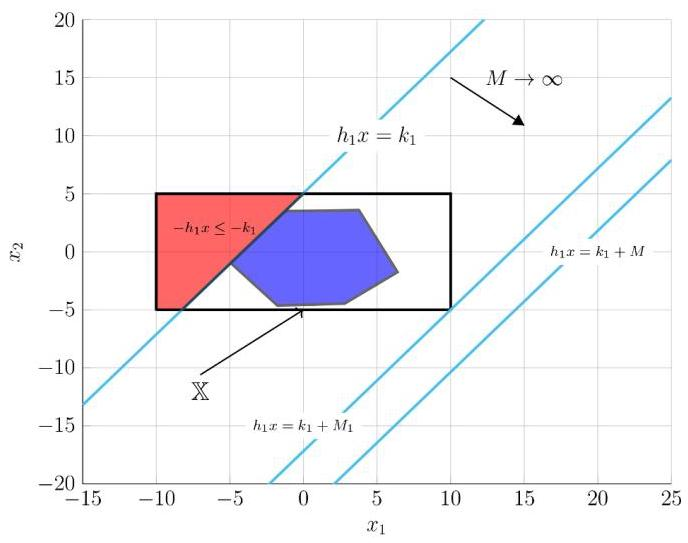
\includegraphics[max width=0.5\textwidth]{images/bo_d55kt477aajc73fvi2bg_3_927_151_688_543_0.jpg}
\caption{“大-M”示意图， \(M\) 如备注4所计算.当约束处于激活状态(即(9a)中的 \({\alpha }_{1} = 0\) )时，所得不等式: \(- {h}_{i}x \leq   - {k}_{i}\) 描述了突出显示的区域.一旦 \({\alpha }_{1} = 1\) (非激活/放宽的约束)，选择 \(M\) 即为放宽的程度.因此，目标是充分放宽，使得其余的约束不受影响.}
\end{figure}


覆盖整个空间的单元超平面排列由所有可行符号元组的集合描述:


\begin{equation}
\mathcal{A}\left( \mathbb{H}\right)  = \mathop{\bigcup }\limits_{{l = 1\cdots \gamma \left( N\right) }}\mathcal{A}\left( {\sigma }_{l}\right) ,
\end{equation}
其中 \(\mathbb{H} = {\left\{  {\mathcal{H}}_{i}\right\}  }_{i \in  \mathcal{I}},{\sigma }_{l} \in  \{  - , + {\} }^{N}\) 是由半空间非空交集产生的符号元组， \(\gamma \left( N\right)\) 是可行单元的数量.

\begin{itemize}\relax
\item\relax 考虑一组障碍物(如图2所示):
\end{itemize}

\[
\mathbb{P} = \mathop{\bigcup }\limits_{{j = 1}}^{N}{P}_{j}
\]

简而言之，收集由(3)定义的相关支持超平面，得到超平面排列(11).将可行单元(10)标记为禁止区域\({\sum }_{\mathbb{P}} = \{ \sigma  : A\left( \sigma \right)  \cap  \mathbb{P} \neq  \varnothing \}\) 或允许区域\({\sum }_{X \smallsetminus  \mathbb{P}} = \{ \sigma  : A\left( \sigma \right)  \cap  \mathbb{P} = \varnothing \}\) ，可以获得可行域的混合整数描述:


\begin{subequations}
\begin{gather}
{h}_{i}x \leq  {k}_{i} + M\left( {1 - {\alpha }_{i}}\right) , \\
- {h}_{i}x \leq   - {k}_{i} + M{\alpha }_{i}, \\
\mathop{\sum }\limits_{{{\sigma }_{l}\left( i\right)  = {}^{\prime } + {}^{\prime }}}\left( {1 - {\alpha }_{i}}\right)  + \mathop{\sum }\limits_{{{\sigma }_{l}\left( i\right)  = {}^{\prime } - {}^{\prime }}}{\alpha }_{i} > 0, \\
\forall {\sigma }_{l} \in  {\sum }_{\mathbb{P}}
\end{gather}
\end{subequations}

\begin{figure}[h]
  \centering
  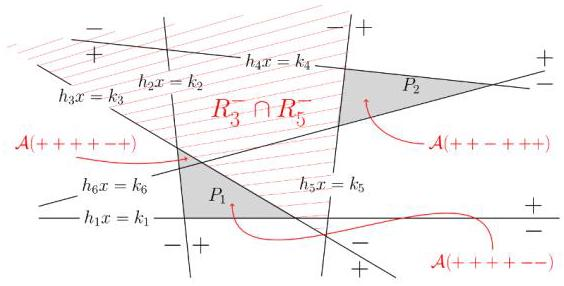
\includegraphics[max width=0.6\textwidth]{images/bo_d55kt477aajc73fvi2bg_3_989_1860_564_286_0.jpg}
  \caption{多面体障碍物与超平面排列.}
\end{figure}

尽管上述提出的构造是一个通用的方案，但表示中的二元部分相当大，因为我们为每个区域都设有一个二元变量(4b).存在多种技术程序，如单元合并(Prodan 等，2015)或对数公式(Vielma \& Nemhauser，2011)，可以用来降低模型的复杂性，但大量的障碍和/或代理仍可能导致二元变量数量过多而不切实际.

被禁止区域的表示不限于多面体集合.例如在 Earl 和 D'Andrea(2005a)中，考虑了如图 3 所示的圆形障碍物，每个由其半径 \({R}_{o}\) 和中心坐标 \(\left( {{x}_{o},{y}_{o}}\right)\) 确定:

\begin{equation}
\mathcal{O} = \left\{  {\left( {x,y}\right)  : {\left( x - {x}_{o}\right) }^{2} + {\left( y - {y}_{o}\right) }^{2} \leq  {R}_{o}^{2}}\right\}
\end{equation}

然而，为了加入相应的避免约束，像(13)中的障碍物被近似为多边形(在 \({\mathbb{R}}^{2}\) 中的多面体，具有 \(p\) 个顶点).因此，每个禁止区域由一组 \({K}_{p}\) 个不等式描述:


\begin{equation}
\left( {x - {x}_{o}}\right) \sin \frac{2\pi m}{{K}_{p}} + \left( {y - {y}_{o}}\right) \cos \frac{2\pi m}{{K}_{p}} \leq  {R}_{o},\forall m = 1,\ldots ,{K}_{p}
\end{equation}

利用(7)中的相同推理和大-M 技术，避免约束被表达为:

\begin{subequations}
\begin{gather}
\left( {x - {x}_{o}}\right) \sin \frac{2\pi m}{{K}_{p}} + \left( {y - {y}_{o}}\right) \cos \frac{2\pi m}{{K}_{p}} \geq  {R}_{o} - M{\beta }_{m},\forall m \\
\mathop{\sum }\limits_{{m = 1}}^{{K}_{p}}{\beta }_{m} \leq  {K}_{p} - 1
\end{gather}
\end{subequations}

\vspace{1 em}
\noindent\textbf{注 5}:除了障碍物的多面体表示外，文献中还考虑了其他表示方法.例如，Ioan、Prodan、Stoican、Olaru 和 Niculescu(2019)通过使用 zonotopic 集合(具有特殊对称性的多面体类别)引入了额外的结构约束.采用此类表示会在模型的复杂性与保真度之间进行权衡.
\vspace{1 em}

值得一提的是，状态空间内的限制可以直接在动力系统建模中处理.特别是在混合系统中，切换(在不同模式间的选择，属于析取型)包含二元变量或离散备选方案.例如，分段线性(PWA)模型代表了一种集成方法，其中非凸域和局部动力学得以统一表达.这种统一建模不同于经典运动规划框架，在后者中，动力学在全局定义，控制决策必须满足非凸的可行域或析取约束.由于我们的综述更偏向于经典运动规划技术，故提及一些相关论文，例如 Bemporad 和 Morari(1999)、Vielma 和 Nemhauser(2011)，这些论文对 PWA 建模工具进行了详尽介绍.\par

\begin{figure}[h]
  \centering
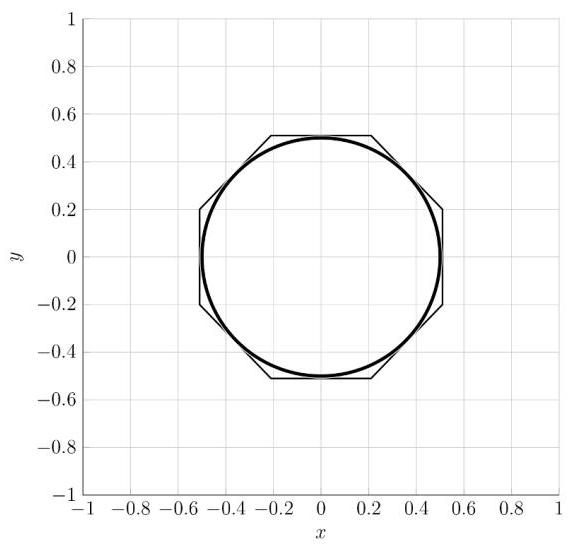
\includegraphics[max width=0.5\textwidth]{images/bo_d55kt477aajc73fvi2bg_4_194_1600_568_545_0.jpg}
\caption{一个圆形障碍物及其多面体近似.}
\end{figure}


\subsection{区域描述的 GDP 公式}

为了突出 GDP 与 MIP 之间的关系，考虑以下示例.我们考虑描述禁止区域的四个支持超平面，并使用 GDP 公式.

因此，对应每个超平面 \(i \in  \{ 1,2,3,4\}\) ，我们有以下析取:

\[
\left\lbrack  \begin{matrix} {Y}_{i1} \\  {g}_{i}\left( x\right)  \leq  0 \end{matrix}\right\rbrack   \vee  \left\lbrack  \begin{matrix} {Y}_{i2} \\  {g}_{i}\left( x\right)  \geq  0 \end{matrix}\right\rbrack
\]

\[
{Y}_{i1} \vee  {Y}_{i2} \leftrightarrow  {Y}_{i2} = \neg {Y}_{i1}
\]

其中 \({g}_{i}\left( x\right)  = {x}_{1} \pm  {x}_{2} \pm  6\) 和我们关联: \({Y}_{i1} =\) 与 \({\mathcal{R}}_{i}^{ - }\) (下半空间)为真， \({Y}_{i2} =\) 与 \({\mathcal{R}}_{i}^{ + }\) (上半空间)为真.禁止区域和允许区域(都在图 4 中示意)可以用以下布尔函数描述:
\begin{itemize}
  \item 凸区域：$\Omega \left( Y\right)  = \neg {Y}_{11} \land  {Y}_{21} \land  \neg {Y}_{31} \land  {Y}_{41}$
  \item 非凸区域：$\Omega \left( Y\right)  = {Y}_{11} \vee  \neg {Y}_{21} \vee  {Y}_{31} \vee  \neg {Y}_{41}$
\end{itemize}

涉及 MIP 公式的集合论工具已被简要概述.欲了解更详细的介绍，读者可参考关于多面体和超平面排列概念的著名著作，如 Ziegler(2012)、Kuhn(1998)，或较新的专著，如 Prodan 等(2015)，这些资料提供了对本文所述概念的更详细数学描述.

\section{运动规划中的 MIP}

运动规划中 MIP 的应用可以源于代数或几何方法.前者涉及涉及逻辑决策的情形，例如从预先已知的备选集中选择.后者通常指 MIP 描述非凸约束的能力.

\subsection*{先决条件}

在进行典型的运动规划MIP实现之前，需要一些澄清.通常，运动规划中存在许多应用，将在第6节中详细介绍.一个重要方面是，所有这些应用都具有由动力学数学模型(线性或非线性)控制的二维或三维空间中质量点的动态行为.

\begin{figure}[h]
  \centering
  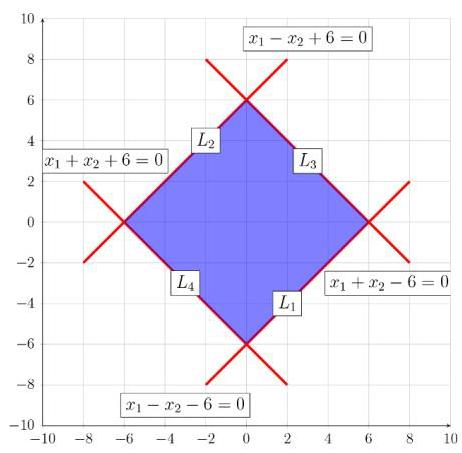
\includegraphics[max width=0.5\textwidth]{images/bo_d55kt477aajc73fvi2bg_4_1039_1695_462_453_0.jpg}
  \caption{GDP公式的示意示例. \({\left\{  {L}_{i}\right\}  }_{i = 1 : 4}\) 超平面.}
\end{figure}

首先，让我们考虑一个由常微分方程(ODE)定义的通用\footnote{文献中存在多种模型变体，但大多可以写成(16)所指定的形式.} 模型，用于受控动力系统:


\begin{equation}
\dot{x}\left( t\right)  = f\left( {x\left( t\right) ,u\left( t\right) ,w\left( t\right) }\right)
\end{equation}
其中 \(x\left( t\right)  \in  {\mathbb{R}}^{{n}_{x}}\) 表示状态向量， \(u\left( t\right)  \in  {\mathbb{R}}^{{n}_{u}}\) 为控制输入向量， \(w\left( t\right)  \in  {\mathbb{R}}^{{n}_{w}}\) 为干扰\footnote{通常，干扰是有界的 \(w\left( t\right)  \in  \mathcal{W}\) ，而 \(\mathcal{W} \subset  {\mathbb{R}}^{{n}_{w}}\) 是凸且紧集.} .映射 \(f\left( {\cdot ,\cdot , \cdot  }\right)  : {\mathbb{R}}^{{n}_{x}} \times  {\mathbb{R}}^{{n}_{u}} \; \times  {\mathbb{R}}^{{n}_{w}} \rightarrow  {\mathbb{R}}^{{n}_{x}}\) 是一个连续函数，具有平衡点(即 \(f\left( {\bar{x},\bar{u},0}\right)  = 0\) ；在不影响一般性的前提下，我们可以假设 \(f\left( {0,0,0}\right)  =\) 为0).

\vspace{1 em}
\noindent\textbf{注 6}:模型(16)描述了连续时间的动态.如下文所述，文献中很大一部分基于离散时间动力学.因此，我们需要同时考虑，保持类似符号，离散时间对应模型:

\begin{equation}
x\left( {k + 1}\right)  = f\left( {x\left( k\right) ,u\left( k\right) ,w\left( k\right) }\right)
\end{equation}

(16)与(17)之间的关联通过多种离散化技术之一实现(Sontag, 2013).在接下来的内容中，前述模型的一个重要特征是选择输入变量的方式以及由此确定的决策域.在文献中，我们可以根据模型的线性/非线性区分这些选择.因此，对于线性模型，参考文献主要集中在状态由位置和速度组成，输入由加速度表示的模型，例如:Bellingham、Richards和How(2002a)；Liu、Dai、Wu和Lin(2017)；Papen、Vandenhoeck、Bolting和Defay(2017)；Richards和How(2002)；Yu、Wang、Bortoff和Ueda(2014).这类模型意味着对每个方向的驱动，通常基于描述受控系统行为的运动学方程.实际上，这种模型有多种变体，源自更复杂的建模技术，但不属于本文讨论范围.关于非线性模型，常用的变体包括状态由位置和航向角组成，输入由速度和转向角表示的模型，例如Rey和Hijazi(2017).

一种常用方法是轨迹跟踪，这隐藏了由避障引起的非线性，但将难点转移到轨迹设计阶段.这可以通过平坦性(在该领域相当流行的方法)来缓解.尽管如此，离线计算轨迹(或路径)假设环境已知，但实际情况可能并非如此.无论线性还是非线性，运动规划中涉及的模型都具有平坦性.一般而言，如果存在一组变量(所谓的平坦输出)，可以在不积分的情况下根据这些变量确定所有状态和输入，则该系统是平坦的，见Murray等人(2009).在Martin、Murray和Rouchon(2002)中，读者可以找到关于这类系统的详细介绍，以及它们在轨迹跟踪或运动规划中的应用.

从控制角度来看，最早的方法主要基于最优控制或非线性规划，但受控系统运行在无障碍环境中.近年来，由于实际原因(尤其是在多智能体环境中)，这种假设已不再适用.因此，控制领域不得不提出一些新技术或对旧技术进行改进.最初的调整是限制受控系统在障碍物周围跟踪预定轨迹，但这些控制策略仅适用于特定系统和环境(LaValle, 2006).

MIP框架在基于优化的控制中经常出现

虽然本文的重点是MIP及其各种实现，但最终，所得到的公式是基于优化控制策略的结果.因此，为了提供关于基于MIP的运动规划问题的总体概述，我们简要介绍一些最优控制理论的概念.

本质上，最优控制问题(Diehl，2014；Kirk，2012)在于找到一个控制输入 \({u}^{ \star  } \in  {\mathbb{R}}^{{n}_{u}}\) ，使系统(16)沿轨迹 \({x}^{ \star  }\left( t\right)  \in  {\mathbb{R}}^{{n}_{x}}\) 运行，同时最小化特定准则:

\begin{subequations}
\begin{gather}
\mathop{\min }\limits_{{x\left( t\right) ,u\left( t\right) }}J = \mathop{\min }\limits_{{x\left( t\right) ,u\left( t\right) }}H\left( {x\left( {t}_{f}\right) }\right)  + {\int }_{{t}_{0}}^{{t}_{f}}L\left( {x\left( t\right) ,u\left( t\right) }\right) {dt} \\
\text{ s.t. }\dot{x}\left( t\right)  - f\left( {x\left( t\right) ,u\left( t\right) ,w\left( t\right) }\right)  = 0 \\
x\left( {t}_{0}\right)  - {x}_{0} = 0 \\
g\left( {x\left( t\right) ,u\left( t\right) }\right)  \leq  0
\end{gather}
\end{subequations}

其中 \(t \in  \left\lbrack  {{t}_{0},{t}_{f}}\right\rbrack  ,\left( {{t}_{f} - {t}_{0}}\right)\) 表示时间范围长度， \({x}_{0}\) 为初始状态， \(g\left( {\cdot , \cdot  }\right)\) 是包含物理约束(如终端或阶段约束)的函数.最优控制问题(18)可以根据i)函数 \(H\left( \cdot \right)\) 和 \(L\left( {\cdot , \cdot  }\right)\) 的选择，例如最短时间问题或终端控制问题(Kirk，2012)；ii)视界( \(\left\lbrack  {t}_{0}\right.\) ， \(\left. {t}_{f}\right)\) )的不同而呈现多种形式，例如Garg等人(2011).

\subsection*{基于MIP的运动规划标准问题}

运动规划问题(LaValle，2006)已被广泛研究，涉及时间最优控制、非线性控制、稳定性、可达性等相关领域.全面回顾这些内容超出本文范围，但我们保留那些明确考虑替代方案或离散决策的部分.重点在于出现非凸可行域并通过混合整数技术编码的具体应用.

本节介绍可以通过MIP方法高效表达的运动规划子领域:
\begin{enumerate}[label=\roman*)]
  \item 任务分配(TA)是将一个目标分配给特定子系统的战略决策(谁去哪里？)，这些目标可以互换，其适用性由特定准则衡量.TA是一个离散决策过程，其中资源-目标配对的备选方案数量是可数的.
  \item 无碰撞路径规划是在位置空间中构建路径，不涉及时间参数化，也不显式考虑动力学.
  \item 无碰撞轨迹规划是构建一个将时间区间与路径关联的函数的问题，考虑了代理的动力学特性，生成的函数以开环方式实现.
  \item (在线)障碍物和碰撞避免是寻找控制输入信号的问题，旨在在最小化性能准则(如18a)同时避免碰撞，并采用闭环策略.
\end{enumerate}

我们在图5中直观展示了上述各项之间的函数关系.值得注意的是，任务分配和路径规划子领域的特殊性在于，动力学的影响通常几乎不影响问题定义，而其他子领域则不同.然而，在某些情况下，动力学会影响静态成本的定义.此外，任务分配和路径规划在大多数运动规划文献中并未作为独立主题单独讨论，而是与其他子领域结合或作为其一部分.如图5(虚线所示)所示，路径规划通常隐含在轨迹规划中，任务分配要么是障碍规避的一部分，要么包含在路径规划中.

\begin{figure}
  \centering
  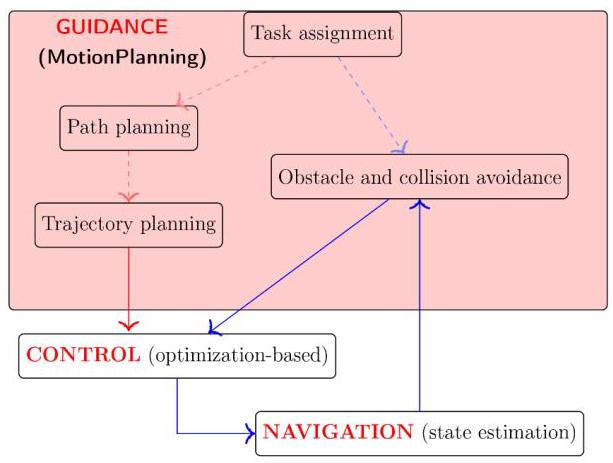
\includegraphics[max width=0.5\textwidth]{images/bo_d55kt477aajc73fvi2bg_6_172_153_613_463_0.jpg}
  \caption{运动规划子领域及其之间的联系.}
\end{figure}


此外，无碰撞轨迹规划和碰撞避免代表两种互补的方法，它们的区别在于与导航和控制的交互方式.障碍规避介入导航-控制环路，而轨迹规划仅生成该环路的参考(待跟踪)信号.

作为补充说明，控制社区中相当一部分也将运动规划中的形成控制包含在运动规划子领域中，尽管它实际上代表一种控制层级，涵盖了上述所有运动规划子领域，并且作为TA，仅在多智能体环境中才有意义.因此，我们在第4节中单独讨论这一主题，介绍多智能体系统中的连通性维护问题.

\vspace{1 em}
\noindent\textbf{注 7}: 在详细介绍运动规划问题之前，有必要强调路径规划与轨迹规划之间的区别.已有大量文献详细讨论这一主题(例如，Beard 和 McLain (2012) 或 Yang、Qi、Xiao 和 Yong (2014)).这两种方法的选择取决于受控系统的具体情况，例如，对于固定翼无人机，轨迹规划方法可能带来一些不良后果(Beard \& McLain, 2012).这些特殊情况在第6节中广泛介绍和讨论.然而，文献中尚未存在对这两个概念的普遍认可的区分.因此，为了简洁起见，我们采用ii)和iii)中的定义. \(\blacklozenge\)
\vspace{1 em}

在表1中，我们展示了关于主要涉及的运动规划问题的参考文献分类.

\vspace{1 em}
\noindent\textbf{注 8}: 一般而言，MIP方法的前提条件是存在一个感知图，涵盖对环境的全局认知.因此，环境的表示对运动规划策略的性能具有重要影响(除任务分配问题外，其影响并不关键).$\blacklozenge$
\vspace{1 em}

\subsection{任务分配}

接下来，我们将介绍一种标准的MIP(混合整数规划)公式，用于任务分配问题，强调其在多智能体系统运动规划中的重要性.


\begin{table}
\centering
\captionof{table}{使用MIP进行运动规划研究的分类.}
\adjustbox{max width=\textwidth}{
  \begin{tabular}{cl}
    \toprule
    应用 & 参考文献(按字母顺序) \\
    \midrule
任务分配 & \makecell{Alighanbari 等人 (2003)；Bethke 等人 (2008)；Chen 等人(2016a)；Chen 和 Wang (2005)；\\Fayazi 等人 (2017)；Haghighi 等人 (2016)；Liu 等人 (2017)；Richards 和 How (2005)；\\Wang 等人 (2015b)；Zhang 等人 (2017a, 2017b)} \\
路径规划 & \makecell{Janecek 等人 (2017a)；Ragi 和 Mittelmann (2017)；Richards 和 How (2005, 2002)；\\Schouwenaars (2006)；Wang 等人 (2015b)} \\
轨迹规划 & \makecell{Ballesteros-Tolosana 等人 (2017)；Cetin 等人 (2007)；Deits 和 Tedrake (2015b)；\\Earl 和 D'Andrea (2002, 2005a, 2005b)；Fayazi 等人 (2017)；Huang 和 Peng (2017)；\\Zhang 等人 (2017b)} \\
障碍与碰撞避免 & \makecell{Bali 和 Richards (2018)；Bellingham 等人 (2002a)；Haghighi 等人 (2016)；Janeček 等人 (2017a)；\\Mukai 等人 (2017)；Rey 和 Hijazi (2017)；Richards 和 How (2002)；Richards 和 Turnbull (2013)；\\Wang 等人 (2015b)} \\
    \bottomrule
  \end{tabular}
}
\end{table}


任务分配指的是将一个目标战略性地分配给特定子系统的决策(它回答“谁去哪里？”的问题).

一般而言，任务分配算法必须提供一个优化特定标准的分配.例如，考虑一次不希望发生的地震，影响了10栋建筑.应急委员会必须为每栋建筑分配救援队，以最小化干预时间，同时考虑救援队的数量及其到达各建筑所需的时间.这个例子可以很容易地改写为多智能体系统中的目标追踪问题.

更一般地，设 \(N\) 个智能体和 \(M\) 个目标.为了最小化到达所有目标的时间，我们应当对智能体与目标进行最优分配.为此，我们定义一个二元变量 \({x}_{ij}\) ，当智能体 \(i\) 访问目标 \(j\) 时取值为1，否则为0.同时，我们考虑每个智能体与目标的相关成本: \({c}_{ij}\) .我们考虑每个智能体必须至少达到一个目标，同时每个目标也必须由某个智能体到达(约束(19b)和(19c)).因此，我们得到了任务分配问题的标准混合整数规划(MIP)模型，如(19)所述.

\begin{subequations}
\begin{gather}
\mathop{\min }\limits_{{x}_{ij}}\mathop{\sum }\limits_{{i = 1}}^{N}\mathop{\sum }\limits_{{j = 1}}^{M}{c}_{ij}{x}_{ij} \\
\text{ s.t. }\mathop{\sum }\limits_{{i = 1}}^{N}{x}_{ij} \geq  1,\forall j \\
\mathop{\sum }\limits_{{j = 1}}^{M}{x}_{ij} \geq  1,\forall i \\
{x}_{ij} \in  \{ 0,1\} ,\;\forall i,j
\end{gather}
\end{subequations}

由于变量 \({x}_{ij}\) 具有整数要求，问题(19)属于整数线性规划(ILP)类别(MIP的一个子类，所有变量均为整数)。值得注意的是(19)的一个特殊特性:求解其线性规划(LP)松弛\footnote{用$x_{ij}\in[0,1]$替换(19d)} 可以获得原始ILP问题的解。然而，如果任务分配问题是增强控制设计的一部分，这一性质将丧失，问题应在(M)ILP的通用类别中求解。例如，定义一个变量 \({t}_{ij}\) ，表示智能体 \(i\) 到达目标 \(j\) 所需的时间。我们要求总时间不超过某个值(20).

\begin{equation}
\mathop{\sum }\limits_{{i = 1}}^{N}\mathop{\sum }\limits_{{j = 1}}^{M}{t}_{ij}{x}_{ij} \leq  T
\end{equation}

在特定情况下，LP松弛可能会导致整数解.

此外，任务分配问题(19)还有许多其他变体.例如，在Smith和Taskin(2008)中，作者考虑了类似的问题，但在成本中引入了非线性项，适用于智能体需要达到多个目标的情况.通过一些细化(详见文中)，他们将问题转化为MILP，尽管其模型比(19)复杂一些.

在Alighanbari等(2003)以及Bethke、Valenti和How(2008)中，针对无人机队的任务分配问题进行了广泛研究.初始要求比(19)中的模型更复杂，因为目标被转化为路径点，每个智能体必须访问一系列这些点.此外，诸如任务耦合或严格时间限制等约束大大增加了模型的复杂性.

另一个例子见于Chen、Shih和Tomlin(2016a)，他们使用任务分配的变体来提供更高级别的控制逻辑，以合成协作安全控制器.实际上，目标是将智能体成对分组，使得相应的规避动作不会导致其他智能体处于危险状态.因此，底层控制器提供的理论保证得以扩展到更多的智能体.

LP模型是NP-hard(非确定性多项式时间难解)(Van Leeuwen \& Leeuwen, 1990).

鉴于MILP的公式是NP-hard，控制领域倾向于通过启发式方法解决此类问题(任务分配或资源分配)，例如在Alighanbari等人(2003)中比较了禁忌搜索与MIP公式，对于高维问题，禁忌搜索表现更佳。然而，MIP公式(19)具有的明显理论优势在于它保证全局最优。这在一些关键情况下具有重要意义.

这在一些关键情况下具有重要意义.

\vspace{1 em}
\noindent\textbf{注 9}: 与任务分配类似，臭名昭著的旅行商问题(TSP)首次出现在Dantzig等人(1954)中，作为MILP提出.对于经典的TSP，采用公式(19)，通过将约束(19b)和(19c)转化为等式，并要求 \(N = 1\) 和 \(M \geq  2\) .
\vspace{1 em}

除了任务分配外，许多资源分配问题也可以直接用MIP公式化.这些问题在相关运动规划领域的多个应用中得到使用，例如飞机维护(或修理)Bajestani和Beck(2013)，机组调度(以及航班重新排程)Mercier和Soumis(2007)等.

存在基于状态空间(工作空间)资源组织思想的方法.更具体地，这些方法将环境划分为等形状的单元格，并将这些单元格视为共享资源.通过这种方式，碰撞和障碍物规避问题被转化为具有互斥关系的资源分配问题.

碰撞规避问题可以被视为具有互斥关系的资源分配问题.

例如，在Wang、Kloetzer、Mahulea和Silva(2015b)中，碰撞规避约束由每个单元格不能被两个不同的代理同时访问的事实给出，即代理不能同时使用相同的资源.该公式是任务分配问题(19)的扩展，创新之处在于以在线方式评估和解决MIP.

使用这种“资源分配”方法的另一个参考是Haghighi、Sadraddini和Belta(2016)，其中机器人群的目标是在二维工作空间中遵循特定且复杂的模式.这些模式通过时空逻辑(SpaTeL)描述.SpaTeL由指示在某一时间访问某个单元格的代理数量的命题组成.这些SpaTeL公式被转化为混合整数线性约束，得到的公式与任务分配(19)类似，但更复杂.Liu等人(2017)也采用了类似的方法，但不同之处在于在运动规划问题中加入了通信约束，形式为信号时序逻辑(STL).

\subsection{路径规划}

如第3节前面所述，路径规划策略涉及生成一条没有明确参数化的路线\footnote{时间未被明确显式化} .此外，这条路线被称为规划路径.

路径规划指在位置空间中构建一条路线，未在时间上进行明确参数化，并且明确考虑系统动力学.

\vspace{1 em}
\noindent\textbf{定义2}:在导航空间中，两点 \({x}_{0},{x}_{f}\) 之间的路径由映射 \(\gamma  : \left\lbrack  {0,1}\right\rbrack   \rightarrow  \mathcal{X}\) 给出，其满足
\begin{equation}
\gamma \left( 0\right)  = {x}_{0},\gamma \left( 1\right)  = {x}_{f}
\end{equation}

有两类方法描述函数$\gamma$，第一类是显式方法，提供整个区间 \(\left\lbrack  {0,1}\right\rbrack\) 内 \(\gamma\) 的值(Janeček、Klaučo、Kalúz和Kvasnica，2017a).第二类是最常用的替代方法，函数必须从一组给定的所谓路径点中取值(Afonso、Galvão和Kienitz，2013).

\vspace{1 em}
\noindent\textbf{注 10}: 路径点代表在无动态环境中的图节点，或是时间区间的边界条件.
\vspace{1 em}

为进一步使用，我们定义描述规划路径的所有路径点集合: \(\mathcal{W} = \left\{  {{x}_{{w}_{0}}\ldots {x}_{{w}_{{N}_{w}}}}\right\}\) ，并在定义2中加入一个附加条件: \(\forall {x}_{{w}_{k}},\exists !{\theta }_{k} \in  \left\lbrack  {0,1}\right\rbrack\) ，使得 \(\gamma \left( {\theta }_{k}\right)  = {x}_{{w}_{k}}\) .

本论文未涉及路径点的选择和确定方法，但在第7节中简要介绍.在路径规划问题中，MIP并不用于生成路径，而是解决路径点的时间分布问题(即它们在路径上的排序)，以满足某些标准.换句话说，MIP在优化通过机器人领域已建立的技术(如采样方法——见第7节)获得的路径中起关键作用.该优化过程的标准必须包括/涵盖由物理和“经济\footnote{在经济MPC的意义上.}”限制所产生的成本.

处理此类问题的最常用方法之一基于任务分配的特殊情况(19)，即旅行商问题(TSP)。在此形式中，我们可以识别出路径规划中对MIP的应用，一个经典的例子见Richards和How(2002)、Schouwenaars(2006)。其中，他们处理一个机器人，需访问 \({N}_{w}\) 个路径点，同时最小化操作成本。因此，强制访问所考虑路径点的MI约束如下:

\begin{subequations}
\begin{gather}
\forall i \in  \{ 1,\ldots ,T\} ,\forall k \in  \left\{  {1,\ldots ,{N}_{w}}\right\}  , \\
\begin{Vmatrix}{{x}_{i} - {x}_{{w}_{k}}}\end{Vmatrix} \leq  M\left( {1 - {b}_{ik}}\right) , \\
\mathop{\sum }\limits_{{i = 1}}^{T}{b}_{ik} = 1,\forall k\text{ and }{b}_{ik} \in  \{ 0,1\} ,
\end{gather}
\end{subequations}

其中 \(T\) 是时间步数， \({b}_{ik}\) 是二元变量，表示路径点 \(k\) 是否在时间步 \(i\) 被访问。约束(22c)确保每个路径点被代理一次。路径点沿区间的排序取决于所选标准(例如，访问所有路径点的最短时间)。实际上，路径点的可达性受到多种因素影响，因此在大多数情况下，接近路径点是合理的目标。在这种情况下，需对(22)进行调整，例如，将约束(22b)替换为 \({H}_{k}\left( {{x}_{i} - {x}_{{w}_{k}}}\right)  \leq  {h}_{k} \; + M\left( {1 - {b}_{ik}}\right)\) ，其中 \({H}_{k}\) 和 \({h}_{k}\) 由描述所考虑邻域区域的支持超平面给出。

\vspace{1 em}
\noindent\textbf{备注11}.在大多数采样基础方法中(LaValle，2006)，寻找最短路径的问题采用多种算法(如Dijkstra、A*)处理。然而，在Taccari(2016)中，作为TSP扩展的基本最短路径问题的几种MIP公式被提出。
\vspace{1 em}

除了依赖于(22)的方法外，还存在一些以不同方式处理基于MIP的路径规划的工作。例如，在Vitus、Pradeep、Hoffmann、Waslander和Tomlin(2008)中，采用了隧道MILP方法。基本上，该算法将全局运动规划问题分为三个主要任务。第一任务是找到一条路径，如定义2所示，同时忽略车辆的动力学约束。接下来，利用路径和空间的凸分解，从起点到目标生成一系列 \({N}_{R}\) 个凸多面体: \({F}_{i} = \left\{  {x \in  {\mathbb{R}}^{2} : {A}_{i}x \leq  {b}_{i}}\right\}  ,\forall i \in  \left\{  {1,\ldots ,{N}_{R}}\right\}\) 。在第三个任务中，这个多面体序列(隧道)被用来限制代理的位置 \(p\left( t\right)\) ，使其沿着从起点到目标的最优且动态可行的路线在隧道内。更具体地说，采用MILP问题，强制代理始终位于隧道的某一区域内。这导致一些OR约束\footnote{解释为异或XOR} ，类似于GDP公式(1)，可以用MI技术直接建模:
\begin{equation}
\mathop{\bigvee }\limits_{{i \in  \left\{  {1,\ldots ,{N}_{R}}\right\}  }}{A}_{i}p\left( t\right)  \leq  {b}_{i},\forall t
\end{equation}

其中 \(p\left( t\right)\) 是考虑的代理的位置.

在Afonso等人(2013)中也采用了相同的思想，其中寻找路径的过程依赖于广义Voronoi图.在这里，考虑了若干点:在障碍物(建模为凸有界集)的面上以及导航环境的边界上，以获得Voronoi图.随后，删除位于禁止区域内的节点及连接这些节点与图中其他节点的边.剩下的图的边形成路径，具有良好的性质，即在距离边最近的障碍物和边本身之间保持相等.这一性质源于Voronoi图构建的本质，即最大化到所有点的最小距离.图中加入起点和终点，保持其连通性.之后，利用Delaunay三角剖分将空间划分为交集为空的三角形(除了它们的边)，该三角剖分依赖于障碍物和已知区域的顶点.计算出穿越规划路径的三角形，并将它们合并成凸多面体，试图在隧道中保持最少的凸区域数.这些多面体随后用于施加障碍物避让约束，如在隧道-MILP公式(23)中所示.

类似的方法中，Deits和Tedrake(2015b)处理了多障碍环境中旋翼无人机的路径规划问题.其基本思想基于混合整数优化，将多项式轨迹分配给凸区域(已知无障碍区域).路径定义为时间上的分段多项式函数，具有向量值系数.预先(离线)选择多项式的次数和段数后，优化问题返回每个多项式的系数，以确保无碰撞轨迹.这种多项式参数化是因为所考虑系统\footnote{纳米四旋翼无人机Crazyflie 2.0.} 的模型具有微分平坦性.关于无障碍的凸区域，它们通过IRIS(迭代区域膨胀，通过半正定规划Deits \& Tedrake(2015a))离线获得，这是一种贪心的空间凸划分技术.所提出的方法在多种仿真场景中进行了测试，结果令人满意，尽管有时凸划分不能覆盖全部无障碍空间.此外，还与经典的\footnote{从作者角度:在生成安全区域时直接使用障碍面(“超平面”).} MIP方法进行了比较，后者可能涉及更复杂的整数规划.这项工作的一个有趣之处在于，生成的路径依赖于所考虑的凸安全区域，用于划分空间.

除了上述工作外，还存在一些边缘性涉及路径规划问题的研究.例如，在Janeček等人(2017a)或Janeček、Klaučo和Kvasnica(2017b)中，介绍了一个工具箱，包含多种辅助工具，用于生成参考路径.因此，提供了已知半径的圆形轨迹或经过给定航点的多边形参考路径，但极少使用MIP.

\subsection{轨迹规划}

轨迹规划涉及确定路径及沿其移动的方法.因此，轨迹规划策略返回一个在时间上明确参数化的路径.本节首先考虑处理一般问题的相关工作，随后关注自主车辆领域的经典应用(如自主超车、合流交叉口或变道).

轨迹规划指在开环中生成的函数，它将时间与路径上的每一点关联起来，并考虑系统动力学的特殊性.

\vspace{1 em}
\textbf{定义3:}在导航空间中的两个点 \({x}_{0},{x}_{f}\) 之间的轨迹由连续函数 \(\gamma  : \left\lbrack  {{t}_{0},{t}_{f}}\right\rbrack   \rightarrow  \mathcal{X}\) 给出，其定义为
\begin{equation}
\gamma \left( {t}_{0}\right)  = {x}_{0},\gamma \left( {t}_{f}\right)  = {x}_{f}.
\end{equation}

\noindent$\blacklozenge$\hspace{1.3em}作为路径规划任务，描述轨迹的连续函数的规范可以用两种不同的方法完成。对于第二种方法，描述轨迹的所有路径点集如下修改: \(\widetilde{\mathcal{W}} = \left\{  {\left( {{x}_{{w}_{0}},{t}_{{w}_{0}}}\right) \ldots \left( {{x}_{{w}_{{N}_{w}}},{t}_{{w}_{{N}_{w}}}}\right) }\right\}\) ，并在定义3中加入额外条件: \(\gamma \left( {t}_{{w}_{k}}\right)  = {x}_{{w}_{k}},\forall {x}_{{w}_{k}}\) 。然而，路径点方法在基于MIP的轨迹规划(以及相关文献)中很少使用。因此，除非另有说明，轨迹通常以连续函数 \(\gamma \left( t\right)\) 明确给出。

处理轨迹规划问题的经典工作之一是Earl和D'Andrea(2005a)，他们提出了一种迭代的MILP算法.更具体地，考虑圆形障碍(见第2.2节，式(13))和传统的非完整(类似汽车)车辆，作者提出了一种算法，保证整个轨迹中的避障，并高效分配避障时间，从而得到更小的MILP模型.

所提出的算法需要对连续非完整模型进行时间离散化.一个有趣的方面是，利用非均匀离散化以避免解决大型MILP所需的繁重计算.支持非均匀时间离散化允许使用智能时间步选择算法，从而生成更高效的MILP模型.因此，迭代MILP算法的思想是找到一种合适的避障时间分布，避免因在每个采样时刻枚举约束而导致的模型复杂度增加.在此，考虑了两类问题:带有障碍规避要求的轨迹生成和最短时间轨迹生成问题.

迭代MILP算法解决了MILP应对大规模模型的问题.

Earl和D'Andrea(2002)的工作研究了多车辆系统的协作控制.在一个简化版本的机器人竞赛要求基础上，作者用混合系统建模了这些简化的竞赛规则.此外，他们将控制问题置于优化框架中，使用MILP.所考虑的简化竞赛涉及两个机器人队伍，攻击者和防御者，在一个中心区域称为防御区的比赛场地上.攻击者是朝防御区飞行的无人机.防御者的目标是通过在攻击者进入防御区前拦截每个攻击者，阻止其进入.一旦攻击者进入防御区或被防御者拦截，它将在比赛剩余时间内保持静止.在追求目标的同时，防御者必须避免与其他防御者和障碍物碰撞，也要避免进入禁止防御机器人的防御区.控制策略由一个集中式控制器实现，该控制器对系统具有完全了解，能即时传输控制信号给防御者.控制器需要确定每个防御机器人所需的输入，以实现目标.利用模型预测控制(MPC)，他们获得了一组控制输入，最小化在演练期间进入防御区的攻击者数量，并且符合系统动力学(机器人动力学)和约束(无碰撞等).所得到的模型是由连续和离散状态组成的混合系统，具有线性动力学，受不等式约束和逻辑规则限制.换句话说，他们获得了一个混合逻辑动态(MLD)系统(Bemporad \& Morari, 1999).最终的优化问题是一个MILP，可以用最先进的求解器(如ILOG CPLEX)轻松解决.

多机器人系统可以用MIP技术建模为混合(MLD)系统.

此外，在Earl和D'Andrea(2005a)中提出了迭代MILP算法，这些算法解决了MILP应对大规模模型的问题.所考虑的问题是具有避障要求的轨迹生成和最短时间轨迹生成问题.这些问题涉及由混合逻辑动力学Bemporad和Morari(1999)方程描述的车辆，这是一种混合系统.该算法比标准MILP方法使用更少的二进制变量，计算量也更小.文中提出的迭代方法适用于由逻辑规则(或状态机)和线性动力学方程混合控制的MLD系统，并通过在障碍场中的车辆验证，这是一种特殊的MLD系统.

在Earl和D'Andrea (2005b)中，汇总并扩展了Earl和D'Andrea (2002)以及Earl和D'Andrea (2005a)的结果.因此，多车辆控制问题采用MILP和MLD系统Bemporad和Morari (1999)进行处理.与Earl和D'Andrea (2002)中一样，这些方法的动力来自于两个机器人团队之间的对抗游戏.一个团队的策略是固定的并由状态机建模，而另一个团队的行为则通过迭代的MILP方法进行控制.顺便提一句，文中所用的方法是独立于Richards和How (2002)中提出的类似方法发展而来的.该论文的一个有趣之处在于，所考虑的环境包含一个对抗性成分，其智能行为通过有限状态机建模，并隐含地使用了MLD系统.

此外，轨迹规划主题在Cetin、Bikdash和Hadaegh(2007)中有所涉及.文中，所解决的问题是为航天器编队的重构生成无碰撞轨迹，同时追求燃料消耗的最优.为了建模航天器的表示及其对应的安全区域，采用未旋转的立方体(一种特殊的多面体表示).此外，轨迹通过三次样条在时间上离散化，因此，通用问题被转化为优化问题.该问题的求解产生了以航天器在一组路径点的位置和速度参数化的轨迹.为此，采用“Big-M”技术将参数化优化写成混合整数线性规划(MILP)，其解可以通过标准的MILP求解器(见第6节)或序贯线性规划的概念获得.文中对这两种方案进行了比较，应用在两个标准验证测试中，目标是在燃料消耗最小的情况下交换航天器内的位置.比较结果引发了关于MILP可行性以及缩短求解时间所需方法的广泛讨论.

此外，Richards 和 How (2003) 使用 MILP 进行开环车辆轨迹设计，允许引入非凸约束，如喷流碰撞规避.

\subsubsection*{自动驾驶车辆中的轨迹规划任务}

轨迹规划中的经典应用大多涉及合流点问题(例如，Bali 和 Richards (2018)；Huang 和 Peng (2017))或自主超车(例如，Ballester-os-Tolosana、Olaru、Rodriguez-Ayerbe、Pita-Gil 和 Deborne (2017)；Molinari、Anh 和 Re (2017)).

自动驾驶领域的最新进展揭示了在辅助驾驶框架下高速公路上的变道和超车等问题.为了执行这些动作，必须计算出符合车辆限制和安全要求的合适且舒适的轨迹.


例如，在Molinari等人(2017)中，提出了一种用于自主超车问题的高效MIP公式.所考虑的车辆具有简单的动力学模型，非凸的可行区域通过类似于Prodan等人(2015)(如第2节)中的超平面排列进行表示.针对被多个车辆包围的代理，提出了一种具有碰撞避免保证的轨迹生成完整公式.MPC准则包含一个期望的参考状态，确保超车的发生.他们还考虑了两种减少二进制变量数量的方法:对数公式和单元合并(Stoican等人，2013).其中的示例以及两种简化方法在复杂度方面的对比分析，在IPG CarMaker(一个精确的车辆模拟器)中得到了验证.

在Ballesteros-Tolosana等人(2017)中，变道和超车动作旨在生成能够确保乘客舒适的轨迹.数学上，该问题被表述为一个最优控制问题(OCP)，因为它处理运动学和碰撞避免约束(后者以超平面排列的形式，如第2节所述).为了减轻这种表示方式带来的巨大计算负担，文中提出了预分析步骤，即枚举所有可能的超车配置及其对应的紧凑MIP形式.通过多次射击法解决所得的非线性约束最优控制问题，相较于预分析步骤，计算负担得到了改善.

合并交汇处问题中存在MIP的情况在大量文献中可以找到.例如，Fayazi等人(2017)研究了自动驾驶车辆在交叉口的最优调度，免除交通信号灯的需求.其思想是设计一个能够协调车辆通过交叉口的控制器，在安全条件下调度交叉口的通行，并接收所有订阅车辆的信息.此外，每辆车会向控制器通报其运动和预期时间表.因此，基于优化的控制器应找到车辆通过交叉口的最优顺序及其对应的通行时间，最小化当前时间与最后一辆车通过交叉口的预期到达时间之间的差异，以及每辆车的分配通行时间与期望时间之间的差距.所得到的优化问题必须考虑一些物理约束(速度限制和最大加速度)以及两辆连续车辆进入交叉口之间的安全“窗口”.这些约束导致了析取和相应的if-then语句，通过MIP(大-M方法)建模.此外，总优化成本由一个极小极大目标和一个非线性成本(绝对值)组成.

MIP可以用来消除非线性(Smith \& Taskin, 2008).

同样，Huang和Peng(2017)解决了信号交叉口的速度轨迹规划问题.其思想是优化多交叉口的车辆速度轨迹，以最小化燃料消耗和行驶时间.为了获得问题的数学模型，作者假设信号交通状态已知，并忽略前车的影响.这种模型的主要优点(相较于例如Fayazi等人(2017))在于考虑了交叉口的转弯(包括转弯速度限制).在对燃料消耗模型、转弯影响和加速度模型进行全面描述后，提出了一个MIP模型.整数变量的引入模拟了在不违反红灯的情况下穿越交叉口，表示绿色相位窗口的激活状态.

此外，Zhang、Su、Sun和Zhang(2017b)提出了一种异质交通网络的控制策略.异质性源于存在信号和非信号\footnote{无信号交叉口遵循先到先行(FCFC)原则.} 交叉口.在验证了所提出的异质交通网络模型后，采用MIP形式提出了控制策略.最后，提供了同质系统与异质系统的比较，为制定系统性规划方法以决定哪些交通交叉口需要信号控制以确保良好的交通控制性能留下了空间.此外，Zhang、Su、Gao和Zhang(2017a)提出了一种考虑车辆和行人存在的交通信号调度策略.在建立了行人流和多交叉口车辆交通网络的数学模型后，调度问题被表述为一个MIQP(混合整数二次规划).

\subsection{障碍物与碰撞避免}

障碍物与碰撞避免是寻找输入控制信号的问题，其目标是在同时避免碰撞的同时，最小化性能指标，如(18a)所示的目标函数，通过闭环策略实现.

一种有效的碰撞和障碍物避免策略变得至关重要，以确保系统和环境的安全与完整性.近年来，控制领域致力于开发能够实现实时操作的无碰撞控制策略.普遍认为，碰撞避免问题具有挑战性，原因在于其非凸可行域的存在.描述这一非凸域具有计算和结构上的影响，通常导致计算效率与控制性能之间的权衡.由于MIP能够像第2节那样明确建模非凸性，它逐渐成为表达碰撞避免问题的合适方法.

在障碍物和碰撞避免问题领域中，MIP 方法可以分为两大类.第一类 MIP 方法更为常用，是非 MIP(机器人)运动规划文献中广泛采用的方法.它包括选择一种不依赖于环境特性的划分方法(例如障碍物的形状).一种标准的划分方式是由等大小的正方形网格组成(Haghighi 等，2016；Wang 等，2015b).采用这种方法，碰撞避免问题在大多数情况下变为资源分配问题，如第3.1节所述.第二类 MIP 方法或几何方法依赖集合论，以及混合整数技术在高效编码非凸集描述方面的能力(见第2节).虽然不同，但两者具有共同特征:工作空间被划分成某种类型的单元，并在某种程度上利用 MIP 来建模析取约束.

\vspace{1 em}
\noindent\textbf{注 12}: 文献中存在区分障碍物和碰撞避免的研究.更确切地说，碰撞避免仅指多智能体系统内的相互碰撞避免，而障碍物避免可能指与静止障碍物或具有已知轨迹(大多为周期性轨迹)的运动障碍物的碰撞避免.同样，部分文献认为障碍物避免指静态环境，而碰撞避免涵盖任何类型的运动障碍物. \(\blacklozenge\)
\vspace{1 em}

\subsubsection*{静态障碍物}

Culligan(2006)的工作提出了一种使用 MILP 的路径规划器，用于解决无人机(UAV)的滚动时域优化问题.该 MILP 公式包括两个重要组成部分:障碍物和多车辆避让的硬约束，以及车辆动力学的近似.还考虑了三维情况，并进行了全面介绍.此外，为了缩短解决时间并增强路径规划器的能力，讨论了对 MILP 框架的若干改进，包括变步长、线性插值点和时域最小化等技术.值得注意的是，变步长的概念被扩展到滚动时域的非迭代 MILP 公式中.变步长允许在不显著增加解决时间的情况下延长仿真时域.时域最小化通过去除不必要的障碍约束来减少解决时间(类似于 Janeček 等，2017a).



在 Schouwenaars(2006)中，作者提出了一个用于在部分未知环境中安全在线轨迹规划的框架.采用 MPC 框架，MILP 在整合碰撞避免约束方面发挥了关键作用(类似第2节中的技术).一个有趣的方面是，智能体可以通过标准(速度)控制系统控制，也可以通过使用允许从离散集合中实现某个机动的机动调度器进行控制.这种混合控制架构被应用并针对特定类型的动力学(对应于小型直升机)进行了增强.此外，关于所提出控制策略的可行性问题也得到了充分处理.因此，提出了一个有益的概念:终端可行不变集，即智能体可以无限期停留在其中且具有反碰撞保证的集合.这些集合是在线计算的，以仿射约束的形式表示在时域的最后状态上.通过这些集合，提供了一个已知的备份方案，具有动态可行性和无障碍性，从而保证了可行性和安全性.该策略在一架无人波音飞机上进行了测试，使用可扩展的盘旋圈作为可行不变集.从多智能体角度看，该控制策略是分布式的，每个智能体只计算自己的轨迹，同时考虑邻近智能体的最新规划行为.潜在冲突在实时中得到解决，以保持可行性保证.为了展示所考虑策略的优势，算法在涉及一群小型直升机的场景中运行，旨在在复杂环境中保持无线连接.

障碍物和碰撞避免约束通常在采样时刻施加，而不考虑智能体在采样间隔内的行为.因此，智能体可能在表面上遵守约束的情况下“转弯绕过”障碍物.文献中采用的思想是考虑额外的约束，以确保两个连续位置之间的线段不会穿越障碍物(Maia 和 Galvao，2009；Richards 和 Turnbull，2013).Stoican、Prodan 和 Grotli(2018)在超平面排列设置中，提供了多障碍物情况的处理方法，包括精确和过度逼近的表示.

\subsubsection*{移动障碍物}

在MIP框架中，移动障碍物不像静态环境那样常见，因为相关的计算负担较重.在大多数涉及时变环境的文献中，受限的移动区域被建模为矩形/立方体排除区域，Richards和How(2005, 2002)如此描述.实际上，这种表示是多面体表示(见第2节)的特殊情况，但对应的混合整数线性约束有限.因此，在二维环境(x-y坐标)中，两个移动障碍物的排除区域约束在MIP中表示为:

\begin{subequations}
\begin{gather}
{x}_{1} - {x}_{2} \geq  d - M{\alpha }_{d1} \\
{x}_{2} - {x}_{1} \geq  d - M{\alpha }_{d2} \\
{y}_{1} - {y}_{2} \geq  d - M{\alpha }_{d3} \\
{y}_{2} - {y}_{1} \geq  d - M{\alpha }_{d4} \\
\mathop{\sum }\limits_{{i = 1}}^{4}{\alpha }_{di} \leq  3
\end{gather}
\end{subequations}

其中 \(d\) 是安全距离(正方形排除区域的边长)， \({\alpha }_{di}\) 是二元变量，而(25e)确保上述约束中至少有一个被激活.值得一提的是，矩形排除区可以用来建模其他非凸约束，例如Richards和How(2005)、Culligan(2006)所述.

与轨迹规划类似，碰撞避免问题也在自主车辆相关任务中得到应用.例如，在Mukai、Natori和Fujita(2017)中，采用MIP结合递归视界策略(MPC)解决高速公路车辆合流问题.因此，受限区域通过逻辑语句(AND/OR)描述，进一步用“big-M”方法建模为混合整数约束.

此外，Molinari等人(2017)使用MPC在高效的MIP框架中处理自主超车问题.所考虑的车辆具有简单的动力学模型，非凸的可行区域如第2节所示.MPC准则包含一个期望的参考状态，确保超车得以实现.

同样，Bali和Richards(2018)提出了一种在交叉口车辆合流场景中基于相对成本优先级的方法.该方法基于MPC，采用MIQP优化.该方案在保证安全和递归可行性的同时，提供了最优控制特性.后者通过简单的时间间隔约束的正控制不变性得以保证.对于两个车辆的示例，验证并展示了可调优的优先级和间隙接受度，并在决策图上呈现.优先级随后在四车辆示例中得到尊重的验证.

\subsubsection*{障碍物避免的等价MLD形式}

混合逻辑动态(MLD)系统首次由Bemporad和Morari(1999)提出，是一种用于建模和控制系统的相关框架，结合了线性动态方程、逻辑规则和操作约束.这些由线性动态方程描述，受线性不等式限制，涉及实数和整数变量，如(26)所示.

\begin{subequations}
\begin{gather}
{x}_{k + 1} = A{x}_{k} + B{u}_{k} + {B}_{2}{\delta }_{k} + {B}_{3}{z}_{k} \\
{y}_{k} = C{x}_{k} + D{u}_{k} + {D}_{2}{\delta }_{k} + {D}_{3}{z}_{k} \\
{E}_{2}{z}_{k} + {E}_{3}{\delta }_{k} \leq  {E}_{1}{u}_{k} + {E}_{4}{x}_{k} + {E}_{5}
\end{gather}
\end{subequations}

其中 \({x}_{k},{y}_{k},{u}_{k}\) 表示系统的状态、输出和输入向量. \({\delta }_{k} \in  \{ 0,1{\} }^{{n}_{\delta }}\) 和 \({z}_{k} \in  {\mathbb{R}}^{{n}_{z}}\) 分别是辅助逻辑变量和连续变量.

考虑一个由单一代理描述的系统，该系统必须在非凸域中移动.该代理由动力学\footnote{为了表达的清晰，以下内容中我们将忽略方程(26b)和(27b)，但推理可以很容易地进行调整.} 描述:

\begin{subequations}
\begin{equation}
{x}_{k + 1} = A{x}_{k} + B{u}_{k}
\end{equation}
\end{subequations}
我们旨在用MLD形式描述所考虑的系统，更具体地，将上述条件重写为(26c)形式.

首先，如果考虑矩阵 \({B}_{2}\) 和 \({B}_{3}\) 为零，则(27a)和(26a)是等价的.接着，将强加的条件 \(\left( {{x}_{k + 1} \notin  P}\right)\) 以类似于(7a)的方式写出，并根据动力学替换 \({x}_{k + 1}\) ，我们简洁地写成\footnote{“0” 表示适合插入位置的零矩阵.} :

\begin{equation}
\left\lbrack  \begin{matrix}  - M{I}_{N} \\  {\mathbf{1}}^{\top } \end{matrix}\right\rbrack  {\alpha }_{k} \leq  \left\lbrack  \begin{matrix} {SA} \\  \mathbf{0} \end{matrix}\right\rbrack  {x}_{k} + \left\lbrack  \begin{matrix} {SB} \\  \mathbf{0} \end{matrix}\right\rbrack  {u}_{k} + \left\lbrack  \begin{matrix}  - R \\  N - 1 \end{matrix}\right\rbrack
\end{equation}

其中 \(M\) 是一个足够大的常数(根据“Big-M”公式)， \(N\) 是描述多面体 \(P = \left\{  {x \in  {\mathbb{R}}^{d} \mid  {Sx} \leq  R,S \in  {\mathbb{R}}^{N \times  d},R \in  {\mathbb{R}}^{N}}\right\}\) 的线性约束的数量， \({I}_{N} \in  {\mathbb{R}}^{N \times  N}\) 是单位矩阵.通过对输入 \(\left( {{S}_{u}{u}_{k} \leq  {R}_{u}}\right)\) 添加约束，所考虑系统的MLD表达式为:

\begin{subequations}
\begin{gather}
{x}_{k + 1} = A{x}_{k} + B{u}_{k} \\
\left\lbrack  \begin{matrix}  - M{I}_{N} \\  {\mathbf{1}}^{\top } \\  \mathbf{0} \end{matrix}\right\rbrack  {\alpha }_{k} \leq  \left\lbrack  \begin{matrix} {SA} \\  \mathbf{0} \\  \mathbf{0} \end{matrix}\right\rbrack  {x}_{k} + \left\lbrack  \begin{matrix} {SB} \\  \mathbf{0} \\   - {S}_{u} \end{matrix}\right\rbrack  {u}_{k} + \left\lbrack  \begin{matrix}  - R \\  N - 1 \\  {R}_{u} \end{matrix}\right\rbrack
\end{gather}
\end{subequations}


\vspace{1 em}
\noindent\textbf{注 13}: 根据Bemporad和Morari(1999)中的定义1，MLD系统(29)是良定义的. \(\blacklozenge\)
\vspace{1 em}

在Ritter、Euler、Ulbrich和Stryk(2014)中，等价的MLD表达式得到了进一步扩展.建模和控制一个多车辆协作系统，使其在合理时间内到达目标位置，避免各个代理之间的任何碰撞.因此，MLD系统是建模多车辆系统的有效紧凑表达，因为所有现有的约束(动力学、碰撞避免、测量等)都嵌入在一个完整的配置中，允许使用现有方法解决控制问题.

\subsubsection*{用于偏差抵消最优控制的MIP重构}

在运动规划中，MIP的另一种应用形式是在DCOC(偏差抵消最优控制)或最优退出时间控制中(Zidek、Bemporad和Kolmanovsky，2017a).此类问题的主要目标是尽可能长时间满足预设的约束(Zidek、Petersen、Bemporad和Kolmanovsky，2017b).换句话说，DCOC是一个特殊的最优控制问题，旨在确定一系列控制输入，以最大化从给定集合的首次退出时间.在运动规划中，DCOC作为一种有用的工具，能很好地处理具有有限资源(燃料或能源)系统的控制问题.在Zidek等人(2017b)中，针对航天器姿态控制的DCOC的MILP表达进行了全面研究，并引入了一种基于LP的迭代方法以求解.

此外，类似的方法中，Maia和Galvao(2009)提出了用于MPC控制器的移动预测时域的实现，解决障碍物避让问题，使用二元变量和隐式的MIP.此外，Richards和How(2003)利用MILP优化实现了可变时域长度，确保了有限时间内的任务完成.

\section{多智能体系统中的MIP: 连通性维护与队形控制}

在当今复杂多变的环境中，大多数活动难以由单一代理/机器人/实体完成，既耗时又困难.因此，为了提高精度、增加冗余并缩短时间，可以采用合作机器人/代理团队.这样，系统安全性和完整性的关键风险因素得以缓解，但也伴随着对被监控和控制系统的广泛扩展.诸如规模庞大、地理分布广、故障率高和异质性等因素，正成为选择合适控制架构的决定性因素.

多智能体系统控制中的一个重要问题是协作团队(机器人)的协调，以高效完成既定的“任务”.在多种情况下，这些智能体团队需要收敛(并保持)特定的空间配置.因此，队形控制通常是运动规划中其他应用的前提条件.

连通性维护指提供约束，确保智能体之间始终保持连通的通信图.

更确切地说，队形的连通性维护通常指反馈律、路径/轨迹规划、碰撞避免和任务分配的集合，保证智能体之间可以通信(以确保数据流，例如控制决策、数据收集、分布式估计等).

\vspace{1 em}
\noindent\textbf{注 14}: 虽然连通性维护和队形控制不是同一现象的不同标签，但其基本思想相似，区别在于全球目标.两者的关键区别在于智能体间相对距离的重要性:连通性维护关注无障碍通信，而距离或相对速度仅在其影响“视线”时相关(例如，距离小于通信范围阈值).
\vspace{1 em}


文献中主要有两种方法解决队形控制问题:Qu(2009)提出的领袖-追随者设计和无领袖方法.前者指定一名智能体为领袖，沿特定方式移动，其余智能体追踪领袖以维持队形.后者通过全局共识协调智能体，以实现整体目标.选择哪种方法取决于团队/智能体的具体情况，即其通信和感知能力.此外，这些方面还影响控制架构，详见第5节.(表2)列出了采用MIP技术进行多智能体系统运动规划策略的参考文献分类.

\subsection{拐角切割规避条件}

拐角切割规避问题是运动规划中一个重要但常被忽视的部分.障碍物和碰撞避免约束通常在采样时施加，而不考虑采样内的智能体行为.因此，智能体可能在表面上遵守约束的情况下“拐角”越过障碍物的角落.

拐角切割旨在提供保证采样内碰撞避免的约束.

其思想简单:智能体只有当其下一位置位于其可见区域(由当前点出发的所有射线的并集，不与任何障碍相交)时，才避免拐角切割.注意，另一种对偶概念(阴影区域——从智能体视角隐藏的区域)可用于强制覆盖整个可行空间，例如画廊问题.

由于精确描述此类区域不切实际，采用混合整数规划(无论是精确还是过度逼近的形式)来实现.在前述超平面排列框架中，这些约束隐式或显式地使用三元符号:智能体的当前位置和未来位置 \(\sigma ,{\sigma }^{ + } \in  {\sum }_{X \smallsetminus  \mathbb{P}}\) ，以及障碍物的坐标 \({\sigma }^{ \bullet  } \in  {\sum }_{\mathbb{P}}\) .

表2

多智能体系统的MIP.

\begin{table}[h]
  \centering
  \caption{多智能体系统的MIP.}
  \adjustbox{max width=\textwidth}{
    \begin{tabular}{cc}
      \toprule
      连接维护 & \makecell{Afonso 等人 (2020)；Earl 和 D'Andrea (2005b)；Richards 和 Turnbull (2013)；\\Schouwenaars、De Moor、Feron 和 How (2001a)；Sun 和 Cassandras (2015)} \\
      编队控制 & \makecell{Bellingham、Tillerson、Alighanbari 和 How (2002b)；Papen 等人 (2017)；\\Prodan、Olaru、Stoica 和 Niculescu (2012)；Ritter 等人 (2014)} \\
      避免拐角切割 & \makecell{Afonso 等人 (2016)；Maia 和 Galvao (2009)；Richards 和 Turnbull (2015)；\\Stoican 等人 (2018)} \\
      \bottomrule
    \end{tabular}
  }
\end{table}


我们已知Afonso、Galvão和Kienitz(2016)；Maia和Galvao(2009)；Richards和Turnbull(2015)关于过度逼近的角落切割约束的讨论，并提供了具体细节:Maia和Galvao(2009)提供了初始构造；Richards和Turnbull(2015)以及Afonso等(2016)分别通过减少必要的约束数量和二进制变量数量来改进它们.Stoican等(2018)进一步提供了多代理在多障碍环境中生成的阴影(及其补集，即可见区域)区域的精确和过度逼近描述.

具体而言，在Maia和Galvao(2009)中，为避免切割单个障碍，必须存在至少一个包含该障碍的半空间，该半空间不包含代理的当前位置和后继位置:


\begin{equation}
\exists i\text{ s.t. }\sigma \left( i\right)  = {\sigma }^{ + }\left( i\right)  = 0.
\end{equation}
由于此类条件常出现在MPC问题中，其中当前位置和后继位置的符号元组都是决策变量，(30)被改写以避免非线性:


\begin{equation}
\mathop{\sum }\limits_{i}\left\lbrack  {1 - {\sigma }^{ \circ  }\left( i\right) }\right\rbrack  {\sigma }^{ + }\left( i\right)  < N + \mathop{\sum }\limits_{i}\left\lbrack  {1 - 2{\sigma }^{ \circ  }\left( i\right) }\right\rbrack  \sigma \left( i\right) ,
\end{equation}
对于所有可能的值 \({\sigma }^{ \circ  } \in  \{ 0,1{\} }^{N}\) .其思想是，在所有约束(31)中，至少有一个可以简化为\footnote{既假设(30)和(31)存在单一障碍物 \(\left( {{\sum }_{\mathbb{P}} = \left\{  {\sigma }^{\bullet ,1}\right\}  }\right)\) ，根据惯例， \({\sigma }^{\bullet ,1}\left( i\right)  = 1,\forall i\) .这意味着 \(\mathop{\sum }\limits_{i}\sigma \left( i\right)  \leq  N - 1,\mathop{\sum }\limits_{i}{\sigma }^{ + }\left( i\right)  \leq  N - 1\) .} (30)，即满足 \({\sigma }^{ \circ  } = {\sigma }^{ + }\) 的那个.

Richards和Turnbull(2015)通过将约束(31)的数量从 \({2}^{N}\) 减少到更易管理的 \(N\) ，改进了Maia和Galvao(2009).这是通过强制两个连续位置 \(x,{x}^{ + }\) 遵守相同的约束实现的，用我们的符号表示为: \(- {h}_{i}^{\top }x \leq   - {k}_{i} + M{\sigma }^{ + }\left( i\right)\) 和 \(- {h}_{i}^{\top }{x}^{ + } \leq   - {k}_{i} + M{\sigma }^{ + }\left( i\right)\) ，对所有 \(i = 1\cdots N\) .这意味着存在至少一个索引 \(i\) ，使得 \(x\) 和 \({x}^{ + }\) 都位于超平面的同一侧(因此在障碍物的相反一侧)，与(30)类似.Afonso等(2016)提出了一种对数方案，以减少参与选择活跃超平面的二进制变量的数量.

这些方法的共同缺点是它们不易处理多代理多障碍的情况.Stoican等(2018)用以下方式推广了(30):

\begin{equation}
\mathop{\sum }\limits_{i}\left| {{\sigma }^{\bullet ,j}\left( i\right)  - \sigma \left( i\right) }\right|  \cdot  \left| {{\sigma }^{\bullet ,j}\left( i\right)  - {\sigma }^{ + }\left( i\right) }\right|  > 0,\forall {\sigma }^{\bullet ,j} \in  {\sum }_{\mathbb{P}}.
\end{equation}
如前所述，当 \(\sigma ,{\sigma }^{ + }\) 都是变量时，(32)变成非线性，因为其中出现了双线性项.因此，可以使用类似(31)的松弛:

\begin{equation}
\mathop{\sum }\limits_{i}\left| {{\sigma }^{\bullet ,j}\left( i\right)  - {\sigma }^{ \circ  }\left( i\right) }\right|  \cdot  \left| {{\sigma }^{\bullet ,j}\left( i\right)  - {\sigma }^{ + }\left( i\right) }\right|  >  - \left| {{\sigma }^{ \circ  } - \sigma }\right| ,\forall {\sigma }^{\bullet ,j} \in  {\sum }_{\mathbb{P}},
\end{equation}

对于所有 \({\sigma }^{ \circ  } \in  {\sum }_{X \smallsetminus  \mathbb{P}}\) ，即当 \({\sigma }^{ \circ  } = {\sigma }^{ + }\) 时，(33)简化为(32).

\subsection{连通性维护条件}

最优动态编队控制是多代理系统领域的热门话题，基于MIP的方法为建模相关约束提供了合适的工具.以下简要介绍由内部因素(如通信)引起的连通性相关主题.

混合整数约束确保每个代理至少在另一个代理的通信范围内.此外，还需避免代理对的孤立，即如果一个代理被强制保持在另一个代理的通信范围内，后者不能被限制在前者的范围内，而应在第三个代理的范围内.为了制定相应的混合整数约束，我们采用Afonso、Maximo和Galvão(2020)的方法.因此，我们考虑一个二进制变量 \({\xi }_{{ij},k} \in  \{ 0,1\}\) ，如果第 \(i\) 个代理在第 \(j\) 个代理的通信范围内，在时间步 \(k\) ，则其值为1，否则为0.接下来，我们可以写出确保 \(N\) 个代理之间通信连通性的约束:

\begin{subequations}
\begin{gather}
\mathop{\sum }\limits_{{i = 1}}^{{N - 1}}\mathop{\sum }\limits_{{j = 1}}^{N}{\xi }_{i,j,k} = N - 1,\;0 \leq  k \leq  T, \\
\mathop{\sum }\limits_{{{v}_{i},{v}_{j}}}{\xi }_{i,j,k} \leq  \# S - 1,0 \leq  k \leq  T,\forall S \subset  V, \\
{\xi }_{i,j,k} = 0,\;1 \leq  i \leq  N,\;1 \leq  j \leq  i,\;0 \leq  k \leq  T.
\end{gather}
\end{subequations}

约束(34b)阻止了可能的对的隔离，强制每个原始通信图 \(V\) 的子图 \(S\) 中至少有一个节点能够与图外的节点通信.此外，结合(34a)保证只能获得连通的通信图(详见Afonso等人(2020)中的定理2)，即保持连通性.

此外，Sun和Cassandras(2015)关注覆盖控制问题.代理团队在二维任务空间中工作，最大化该空间的覆盖.形成控制采用领袖-跟随的视角，领袖沿给定轨迹移动，其余代理必须保持队形.因此，队形在领袖开始沿轨迹移动时变得动态，必须适应任何环境变化(新任务、新队伍组成或检测到的障碍).首先，简要提出一个通用最优队形问题的公式，将其作为一个优化问题，其目标函数依赖于代理的空间位置.优化问题的约束由位置的可行空间(包含在二维任务空间中)和无向图必须连通的条件组成.该图模拟代理之间的理想连接.可行空间可以是凸的(无障碍)或非凸的(有障碍)，这使得图约束的处理变得复杂.因此，这两种情况必须分别处理.对于凸的可行空间，最优动态队形问题被重写为一个MINLP，通过引入一组在无向图上的流变量(为每两个代理之间的连接关联一个整数流量).问题中的约束被转化为一组混合整数不等式.同时，避免了在所有时刻重新求解MILP的高计算负担，提供了在一定时间区间内保持最优队形的充分条件.对于非凸的可行空间，问题采用不同的方法解决.在每一时刻，当连接丧失时，构建一个新的无向连通图，使得维持初始队形的努力最小.开发了构建新图的算法，并将其作为CPA(连通性保持算法)的输入.文中还考虑了第二种情况的示例，其中初始队形通过凸可行空间的MILP计算，之后考虑障碍物.

\subsection{由外部约束引起的连通性}

本节介绍在队形控制中遇到的目标类型/目标，这些目标由外部\footnote{关于多智能体系统.} 因素强制执行.

在由移动传感器组成的特定区域高效覆盖问题中，连通性维护是由外部因素引发的经典例子之一.例如，Ritter等人(2014)针对由多个配备传感器的自主车辆组成的移动传感器平台解决了这一问题.提出了一种基于模型和多智能体协作系统的在线估算扩散过程状态的自适应观测策略.多车辆协作系统采用MLD系统建模(Bemporad \& Morari, 1999)；控制目标是在合理时间内到达目标位置，同时避免代理之间的碰撞.代理的目标位置通过基于偏微分方程(PDE)的状态估计\footnote{偏微分方程.} 获得，更准确地说，是最优测量位置.因此，MLD系统是建模多车辆系统的良好选择，因为所有现有的约束(动力学、碰撞避免、测量等)都嵌入在完整的配置中，允许使用标准方法解决控制问题.



此外，一个常见的问题是会合操作，多个代理(通常是一支航天器队伍)必须在最短时间内达到特定的队形.Papen 等人(2017)针对包含静态和动态障碍物的环境中的固定翼无人机队伍处理了这个问题.控制策略通过分布式架构实现(具体来说，应用于每个代理的MPC)，每个代理只知道自己的轨迹(由当前位置和速度定义).通过引入二进制变量来建模障碍物并消除一些非线性约束(如速度和加速度约束)，将MPC优化问题转化为MILP.值得注意的是，每个无人机后方形成的湍流尾涡被建模为动态障碍物，因为在这些区域内难以控制无人机.求解由此产生的MILP需要相当的时间，但通过放宽一些约束和细致调优，复杂度得以限制.

\section{控制架构}

目前有三类成熟的控制架构，已在各种应用领域得到广泛研究:集中式、分布式和去中心化.后两者要求局部控制器仅优化其局部输入，计算负担相似.这两者的区别在于通信的影响，去中心化控制不需要代理之间的通信.

在本文中，识别/讨论控制架构在运动规划领域的优缺点不在范围之内，因此，我们只关注它们与MIP的结合方式.在表3中，我们划分了基于MIP的运动规划参考文献，按照控制架构和涉及的代理数量进行分类.

值得一提的是，除集中式外，其他架构中采用的控制策略多为基于优化的方法，偏好MPC.因此，本节重点介绍具体的MPC实现方式.然而，我们也没有忽视那些在分布式/去中心化非MPC策略中使用MIP的文献，因为它具有制定任务分配问题的能力.这些内容在第3.1节中有详细讨论.

涉及MIP的控制架构自然由集中式逐步演变到去中心化和分布式策略.

\begin{table}[h]
  \centering
  \caption{运动规划中MIP方法的分类.}
  \adjustbox{max width=\textwidth}{
\begin{tabular}{|c|c|c|c|c|}
\hline
代理 & 集中式 & 去中心化 & 分布式 & 参考(例如) \\
\cline{1-5}
\(N = 3/ \; N \geq  3\) ，部分 &  \ding{51}  &  \ding{56}  &  \ding{56}  & Chen 等人 (2016a) \\
\cline{1-5}
\(1\ldots N\) &  \ding{51}  &  \ding{56}  &  \ding{56}  & \makecell{ Earl 和 D'Andrea (2005b)；Haghighi 等人 (2016)；Janeček 等人 (2017a)， \\ Ritter 等人 (2014)；Sun 和 Cassandras (2015) } \\
\cline{1-5}
\(1\ldots N\) &  \ding{51}  &  \ding{51}  &  \ding{56}  & Wang 等人 (2015b) \\
\cline{1-5}
\(1\ldots N\) &  \ding{56}  &  \ding{56}  &  \ding{51}  & Papen 等人 (2017) \\
\cline{1-5}
\(N = 1\) &  \ding{51}  &  \ding{56}  &  \ding{56}  & Molinari 等人 (2017)；Ragi 和 Mittelmann (2017) \\
\cline{1-5}
\hline
\end{tabular}
}
\end{table}

\subsection{集中式}

由于其理论上的简洁性，集中式方法是控制多代理系统最常用的方式.在这种架构中，整个多代理系统被视为一个整体，相当于一个扩展的单一代理系统.物理限制(如通信限制)被完全忽略，每个代理只需了解其他代理的行为/动作，所有信息都集中在单一的全局控制器中(Rawlings 和 Mayne，2009).然而，这种方法有限制，不仅因为不可避免的物理约束，还因为由系统复杂性带来的数值难题，这些都由扩展系统的庞大复杂性引起.



注意: \(\left( \checkmark \right)\) 已处理， \(\left( \times \right)\) 未处理， \(\left( {1\ldots N}\right)\) 任意数量的代理

如第3节所述，在文献中，MIP可能出现在不同的控制层级.例如，在Chen等人(2016a)中，碰撞避免问题针对多智能体系统(最少 \(N = 3\) 个智能体)进行处理.他们考虑 \(N\) 个智能体，每个具有类似的动力学和 \(N -\) 个所谓的危险区域: \({\mathcal{Z}}_{ij}\) .每个智能体使用两个控制器:“生存控制器”帮助完成智能体自身的目标(例如到达目标)，而“安全控制器”则必须让智能体远离其他智能体的危险区域.“安全控制器”的架构是集中式的，保证对于 \(N = 3\) ，每个智能体都不会进入任何其他的危险区域.在此，MIP被用来提供更高层次的控制逻辑，以合成合作的“安全控制器”.目标是将智能体配对，使相应的规避动作不会导致对其他智能体的危险情况.

对于通用的障碍物和碰撞避免问题(在 MI-MPC 框架第 3.4 节中)，在对应的全局系统最优控制问题(OCP)中，个体代理的动态行为通过成本函数和约束相互耦合.此外，所有其他代理都可以获得每个代理动力学(由方程描述)的完全知识.因此，全球模型将在预测控制的背景下使用，允许使用非凸约束以实现碰撞避免行为.

作为一个非MPC的示例，Wang等人(2015b)研究的问题是多机器人系统中的碰撞避免。该方法与前述论文之一(Haghighi等人，2016)颇为相似。工作空间被分解为形状相同的单元格，且每个单元格不能同时被两个机器人访问。每个机器人必须通过从一组可能的轨迹中进行选择来完成其任务。这些轨迹由一系列相邻的单元格以及穿越时间（即智能体通过相应单元格的时间）来描述。在此表述下，碰撞避免问题转化为资源分配问题（单元格可视为共享资源）。假设智能体的控制是独立的（即它们不能为了让路或获得优先权而暂停移动），本文提出的思路是为每个智能体计算一个初始延迟时间，以确保不发生碰撞。在集中式控制策略中，轨迹由中央单元选择。因此，控制算法除了返回初始时间延迟外，还必须返回一条“最优”轨迹，而目标保持不变。相关的优化问题是MIP，其中二进制变量用于对由相应资源分配问题产生的析取关系进行建模。值得注意的是，目标函数是一个极小极大（minmax）问题，因为假设机器人并行工作，完成移动的最短（min）时间取决于最慢（max）机器人的时间。该目标可以通过例如Smith和Taskin(2008)中的工具重新表述为标准的最小化问题。



虽然在最坏情况下，MIP 公式的复杂度会随着二进制变量数量的指数增长，但在全局系统维度较高的情况下，MIP 在实时实现中的可靠性会降低.无论公式的效率如何，代理数量的增加也存在同样的缺点.

\subsection{分布式}

分布式控制方法的基本思想，Maestre、Negenborn 等人(2014)提出，是将全局控制问题划分为若干子问题，每个子问题涉及一组特定的局部控制器或代理.因此，每个代理无法获得全局信息，但可以部分了解局部子系统其他组件的行为.

在大规模多智能体系统中，智能体分散在给定的工作空间内，处理一组较小和/或较简单的问题比应对复杂的全局系统更为方便.整体控制策略由局部控制器的行为决定，可能具有合作交互.与集中式架构相比，有几个优点:例如，复杂度降低和可扩展性.然而，性能和全局稳定性的丧失可能变得明显，难以像集中式方法那样保证.将系统解耦为独立节点、设计鲁棒控制策略、寻求共识，所有这些都试图解决问题，但成功有限 Cao, Yu, Ren, and Chen (2012).

在MIP框架下，已提出大部分采用MPC策略的分布式控制方法.MPC的特性使得可以明确处理不同子系统/代理之间的交互.例如，在Schouwenaars (2006)中，采用分布式MPC策略导航一支车辆队伍穿越部分未知的杂乱环境.

由于固有的复杂性问题，以及隐含的缺乏可扩展性，MIP曾不是分布式架构的常用方法.然而，控制界对分布式MIP求解算法给予了特别关注.例如，Testa、Rucco和Notarstefano (2017)提出了一种解决MILP的算法，其中约束分布在各个代理之间.同样，Vujanic、Esfahani、Goulart、Mariéthoz和Morari (2016)基于拉格朗日对偶性，提供了一种特别适用于大规模MILP的分解方法.此外，还有一些工作使用MIP技术来制定问题，并采用启发式方法进行求解，例如，Van Parys和Pipeleers (2016)使用交替方向乘子法(ADMM).

\subsection{分散式}

在过去的几十年中，多智能体系统的分散控制因其广泛的应用而受到极大关注，包括多机器人系统、交通运输、多点监控和生物系统.多智能体导航在机器人和控制领域都是一个重要研究课题，因其需要在同一工作空间内实现多机器人自主控制.多智能体导航的重要应用还包括空中交通管理和自动驾驶，确保与其他车辆和障碍物的碰撞避免.

如前一小节所示，修改控制架构的主要动机之一是集中式问题的计算负担.最初的改动是将问题分解(“分布”)，并期望通过求解子问题达成共识.进一步推进，若不追求达成共识，则形成分散式策略(“各自为战”).在此策略下，每个代理拥有一个控制器，独立行动，不考虑其他代理的行为信息.此外，信息交换有限(大多数情况下，最小化).

去中心化方法的一个基本示例是 Bali 和 Richards (2018) 提出的\footnote{无信号交叉口.} 问题.在集中式(或构建良好的分布式)方法中，每当两个(或更多)代理到达交叉口时，会根据明确的标准进行优先级排序.对于去中心化方法，由于通信有限且无法保证最优，最可能的情况是系统陷入死锁.换句话说，去中心化方法通常无法提供集中式和分布式方法所具有的理论保证.然而，在实际中，去中心化方法可能会带来高效的策略，避免其他方法的计算负担；但对其敏感方面的理解绝对必要.

例如，回想Wang等人 (2015b) 在第5.1节中提到的多机器人系统中的碰撞避免问题.采用分散控制策略时，他们假设每个代理独立选择其轨迹(来自预先已知的集合)，不通知其他系统.在这种情况下，碰撞避免策略应考虑所有可能的轨迹组合，并返回初始时间延迟，以确保在最短时间内完成运动且无碰撞.所得优化问题为MIP，与集中式情况相同.

\section{使用MIP的控制应用}

虽然前几节涉及建模和控制问题，本节将介绍一些关键细节，涵盖本文所提出方案的计算机仿真和硬件实现方面的内容.

值得一提的是，目前尚无明确且无争议的指南能为特定问题生成最优的MIP表达式.一个表达式的性能\footnote{计算时间、可行性等.} 通常高度依赖于具体的软件工具或硬件平台.接下来将简要介绍这些方面，重点在于不同实现方案之间的差异及其对运动规划实际性能的影响.

\subsection{MIP软件}

如前所述，MIP因其建模能力和专用求解器的可用性，是规划与控制问题的强大工具.在过去十年中，开发专门的MIP求解器的努力不断加强，以缓解由整数/二元变量引起的数值问题.

优化建模语言是将数学表达转化为求解器可解形式的工具箱.

在进一步操作之前，我们应强调优化建模语言与求解器之间的区别.前者指的是与后者交互的工具箱/包/库:将受约束优化问题的数学模型转化为内部形式，然后进行求解，并检索和显示其后续结果.注意，大多数现代工具会进行预处理步骤(可能减少二进制变量的数量)甚至自动将问题转化为MI形式(例如，在YALMIP中指定互补条件或双层程序时).



多样的编程语言和在线资源促进了MIP问题的规范和解决.除了经典的Matlab外，最近优化控制社区的关注点转向了Python或Julia等其他先进的编程语言，这些语言已变得对更广泛的科学和工程界更易获取.在表4中，我们总结了这些编程语言、建模语言以及可以结合使用以解决MIP的求解器.

不详尽列举，但有一些流行的优化建模工具:YALMIP(Lofberg，2004)、MPT(Herceg，Kvasnica，Jones \& Morari，2013)、AMPL(Fourer，Gay \& Kernighan，1987)、CVXPY(Diamond \& Boyd，2016)、PYOMO(Hart 等，2017)或 JuMP(Dunning，Huchette \& Lubin，2017).它们都是\footnote{除了AMPL}开源的建模语言，允许用户用高级(几乎是代数或伪代码)语法表达各种优化问题(不仅限于MIP).如表4所示，每种建模语言的开发都考虑了特定的编程语言特性.注意，这些建模工具之间的层级很大程度上取决于用户/研究者的经验，对其中某一工具的偏好对解决性能(例如计算负担)几乎没有影响.这些性能更多受到求解器选择与问题表述方式的关系影响.

关于求解器，存在多种选择，我们在此提及在MIP运动规划领域中最常用的有CPLEX(2009)、Inc.(2014)或Mosek(2015).例如，Huang和Peng(2017)；Zhang等(2017b)或Mukai等(2017)使用GUROBI，而Richards和How(2002)、Schouwenaars、Richards、Feron和How(2001b)或Earl和D'Andrea(2005a)则采用CPLEX.

\vspace{1 em}
\noindent\textbf{注 15}: 大多数求解器(见表4)能够处理二次目标和/或约束，这些元素在许多控制策略和/或应用中具有重要影响，例如(18).
\vspace{1 em}

虽然对求解器所采用的求解技术的综述超出了本文范围，但我们只提及核心技术:分支定界和切平面算法.存在多种变体，各有优缺点.例如，分支切割法(Stubbs \& Mehrotra, 1999)结合了分支定界和切平面算法的优点，通过迭代引入约束以裁剪可行区域，从而减少搜索树中的节点数.



\begin{table}[h]
  \centering
  \caption{MIP实现软件示例.}
  \adjustbox{max width=\textwidth}{
\begin{tabular}{|c|c|c|}
\hline
软件 & \phantom{X} & 参考文献(例如) \\
\cline{1-3}
\multirow{3}{*}{编程语言} & MATLAB & Bemporad 和 Mignone (2000)；Culligan (2006)；Janeček 等 (2017a) \\
\cline{2-3}
 & Python & Welder 等 (2018) \\
\cline{2-3}
 & Julia & Lubin、Yamangil、Bent 和 Vielma (2018) \\
\cline{1-3}
\multirow{7}{*}{建模语言} & Yalmip & Mukai 等 (2017)；Zhang 等 (2017b) \\
\cline{2-3}
 & GAMS & Lee 和 Grossmann (2000) \\
\cline{2-3}
 & CVX/ & Dueri 等 (2017) \\
\cline{2-3}
 & CVXPY & \phantom{X} \\
\cline{2-3}
 & Pyomo & Legg 等 (2012) \\
\cline{2-3}
 & JuMP & Welder 等 (2018) \\
\cline{2-3}
 & AMPL & Richards 和 How (2005, 2002) \\
\cline{1-3}
\multirow{3}{*}{求解器} & CPLEX & Janeček 等 (2017a)；Stoican 等 (2013) \\
\cline{2-3}
 & GUROBI & Janeček 等 (2017a) \\
\cline{2-3}
 & SCIP & Berthold 等 (2012) \\
\cline{1-3}
\hline
\end{tabular}}
\end{table}


一般而言，求解器可以根据不同标准进行分类，例如凸/非凸、启发式/确定性.文献中有更详细的综述，例如 Belotti 等人(2013)对该主题的研究，但从本文的角度来看，相关的方面是:一些现有且可靠的求解器可能采用启发式方法以加快标准算法的速度.这在复杂(大型)问题和实时求解中尤为必要.需要提醒的是，由于启发式的使用，不同求解器的性能(尤其是计算时间)可能差异很大.因此，我们认为“最佳MIP求解器”的概念毫无意义.更积极的一面是，我们观察到对于任何给定问题，都能找到能够解决它的求解器.

除了这些强大的商业求解器外，还存在各种非商业/开源求解器，能够提供合理的性能，在某些情况下甚至优于商业求解器.这类求解器的一个重要特性是，它们的调整和适应能力可以比商业求解器更快、更直接地应对实际应用中的挑战和实时控制需求，后者还需考虑商业因素、免费与付费功能的平衡等.例如，SCIP(https://scip.zib.de)(Achterberg，2009)最初是一个实现了分支定界算法和多种启发式的MILP求解器，而后续版本能够解决带二次目标的MINLP、非凸MINLP或MISDP(混合整数半正定规划)问题.

此外，控制领域的一部分研究者集中关注(如表5所示)对标准MIP求解算法的改进技术.例如，Bemporad、Mignone和Morari(1999)提出了一种高效的分支定界算法，优化了树搜索策略.其应用涉及MLD系统的控制和状态估计(Bemporad \& Morari，1999).类似地，Bemporad(2015)提出了一种结合经典分支定界和非负最小二乘(NNLS)方法的算法，用于解决由混合模型预测控制(MPC)产生的MIQP问题.该思想在Naik和Bemporad(2017)中得到了进一步发展，将NNLS替换为加速对偶梯度投影算法.

还有一些工作利用分支定界算法中的问题结构特性.例如，Feng、Villanueva、Chachuat和Houska(2017)提出了一种变体——分支提升算法，在解决经典障碍物避让问题时表现更优.同样，Hespanhol、Quirynen和Di Cairano(2019)提供了一种迭代变体的分支定界算法，利用问题的块稀疏最优控制结构以及前一时间步的相关信息.

顺便提一句，除了标准的MIP求解算法外，文献中还存在一些启发式(见表5)技术.这里不作详尽列举，仅提及其中两个\footnote{最常遇到的.}:


\begin{table}[h]
  \centering
  \caption{用于MIP求解的替代和启发式技术.}
  \adjustbox{max width=\textwidth}{
\begin{tabular}{cc}
\toprule
备选 & 参考文献 \\
\midrule
分支界限法 & Bemporad (2015); Bemporad 和 Mignone (2000); \\
变异 & \makecell{Bemporad 等人 (1999); Feng 等人 (2017); Hespanhol 等人 (2019);\\ Naik 和 Bemporad (2017)} \\
ADMM & \makecell{Abboud 等人 (2015); Kanno 和 Kitayama (2018); Scott 和 Thiébaux (2014);\\ Takapoui 等人 (2020); Timotheou 等人 (2014)} \\
FP & Fischetti 等人 (2005); Fischetti 和 Salvagnin (2009); Miertoiu 和 Dumitrescu (2019) \\
\bottomrule
\end{tabular}}
\end{table}

\begin{enumerate}[label=\roman*)]
  \item 基于ADMM(交替方向乘子法)的方法 Kanno 和 Kitayama (2018)，Takapoui、Moehle、Boyd 和 Bem-porad (2020).虽然是一种求解凸优化问题的算法，ADMM 也被证明是一种有效的近似解决某些非凸问题的方法.启发式方法的思想是多次用随机初始点重启ADMM，在大多数情况下，这能以较低的计算成本提供可接受的解.这一技术常用于最优(功率)潮流问题，例如交通信号控制 Timotheou、Panayiotou 和 Polycarpou (2014) 或网络 Abboud、Bastuğ、Hamidouche 和 Debbah (2015)；Scott 和 Thiébaux (2014).然而，Van Parys 和 Pipeleers (2016) 在多车辆系统的运动规划中采用了ADMM.此外，该技术存在多种变体和改进.例如，Stellato、Naik、Bemporad、Goulart 和 Boyd (2018) 开发了一种新颖的分支界限算法，专为基于ADMM的求解器量身定制.
  \item FP(可行性泵)Fischetti、Glover 和 Lodi (2005).一种用于寻找给定MIP的可行解的启发式方法，FP旨在最小化LP松弛解与原始MIP解之间的差异.例如，Miertoiu 和 Dumi-trescu (2019) 使用并改进了该算法以适应稀疏表示.
\end{enumerate}

\vspace{1 em}
\noindent\textbf{注 16}: 除了求解器和建模语言外，文献中还存在如Janeček等人 (2017a) 提供的用于障碍物规避问题的MPC控制工具箱.该工具箱采用面向对象的方式开发，便于快速建立相关的MPC问题，并随后为任何非专业用户提供高效的底层优化问题的表达.换句话说，OPTIPLAN工具箱封装了与MIP问题的建模和求解相关的所有方面.
\vspace{1 em}


\subsection{硬件平台}
在详细介绍之前，值得一提的是，部分现有工作考虑了硬件平台的特殊性，开发了特定的方法，而大多数其他工作则提出了通用方法，能够(或不能)适应构造约束.

存在多种机器人平台，广泛应用于学术和/或商业领域:空中、地面或水下车辆.通常，这些机器人参与的活动对人类来说是危险或困难的.尽管可以实现不同程度的自主性，但控制领域普遍偏好无人车辆.主要原因是消除或减轻人为风险.这一方面对成本效益具有积极影响，并且在大多数情况下也提高了操作的准确性.

在表6中，我们展示了用作MIP运动规划问题硬件平台的无人车辆类别:无人机(UAV)、无人水面艇(USV)、无人地面车辆(UGV)或无人水下潜航器(UUV).每一类(或有时是子类)车辆的具体特性带来了不同的运动规划设计挑战.例如，USV/UGV在二维工作空间中移动，而UAV和UUV在三维空间中，因此控制问题的复杂度更高.另一分类依据是车辆是否能停止和/或倒退，例如，固定翼无人机需要保持最低速度(以避免失速)，而四旋翼/直升机(旋翼无人机)具有更多自由度，可以保持任意速度(甚至悬停在空中).

\begin{table}[h]
  \centering
  \caption{硬件平台的分类.}
  \adjustbox{max width=\textwidth}{
\begin{tabular}{cc}
\toprule
实验平台 & 参考文献 \\
\midrule
无人机 & \makecell{Bellingham 等人 (2002a, 2002b)；Chen 等人 (2016a)；Culligan (2006)；\\Papen 等人 (2017)；Ragi 和 Mittelmann (2017)；Rey 和 Hijazi (2017)；\\Richards 和 How (2002)；Schouwenaars (2006)} \\
地面机器人 & \makecell{Bali 和 Richards (2018)；Ballesteros-Tolosana 等人 (2017)；\\Fayazi 等人 (2017)；Molinari 等人 (2017)} \\
\bottomrule
\end{tabular}}
\end{table}


例如，在Culligan(2006)中对MILP框架进行了实验验证:在室内四旋翼测试平台上的试飞展示了该方法在最优路径规划中的可靠性.例如，使用MILP路径规划器在十秒后制定计划，四旋翼可以在MILP求解时间不到一秒的情况下穿越障碍丰富的场地.在无障碍环境中，简单的规划在50毫秒内即可完成.还通过多车辆测试展示了使用MILP进行非通信冲突轨迹规划的能力.

在精准农业、灾害管理和目标追踪等许多应用中，假设无人机与地面传感器协作.无人机作为移动汇点:延长传感器的寿命(通过取消其与基站通信的需求 Xu、Xiao、Yang、Cuthbert \& Wang(2018))，并降低运营成本(通过取消对人工监督的需求 Jawad、Nordin、Gharghan、Jawad \& Ismail(2017)).这些应用在运动规划中引入能量限制，可能由路径长度 Khan 和 Kumar(2016)或通信需求 Xu 等(2018)引起.此外，许多工作通过假设预定义路径原语(例如，无人机限制在直线或平行线 Wang、Ma、Yan、De 和 Das(2015a))或螺旋线 Yue 和 Jiang(2018))简化运动规划.当环境杂乱或不平时，信号衰减可能导致通信链路减弱或丢失 Jawad 等(2017).因此，必须考虑在航点的通信时间限制，这对固定翼无人机来说较难处理.如其他地方所述，这导致一个非线性(在成本和约束方面)受约束的优化问题，通常难以求解.即使是确保悬停在航点的简单要求，也会形成一个MINLP(Mathur、Nielsen、Prasad \& Prasad，2016).

\section{MIP的替代方案}

本节简要介绍在运动规划问题中广泛使用的MIP替代方案.我们在表7中列出了这些替代方案的最新研究参考.


\begin{table}[h]
  \centering
  \caption{运动规划中MIP替代方案的分类.}
  \adjustbox{max width=\textwidth}{
\begin{tabular}{cc}
\toprule
方法/技术 & 参考文献 \\
\midrule
基于图的算法 & \makecell{ Hsu 等人 (2007)；Karaman 和 Frazzoli (2011)；Ladd 和Kavraki (2004)；\\LaValle (2006)；Lozano-Pérez 和 Wesley(1979)；Weiss 等人 (2017)} \\
势场公式 & \makecell{ Chen 和 Wang (2005)；Filotheou 等人 (2018)；Rimon 和 Koditschek (1992)；\\ Vlantis、Vrohidis、Bechlioulis 和 Kyriakopoulos (2018)；\\Vrohidis、Vlantis、Bechlioulis 和 Kyriakopoulos (2018) } \\
凸松弛 & \makecell{ Liu 和 Lu (2014)；Mao 等人 (2017, 2016) Harris 和 Açıkmese (2014)，\\Rey 和 Hijazi (2017) Frasch 等人 (2013)；Janeček 等人 (2017a)；\\Yu 等人 (2014) } \\
\bottomrule
\end{tabular}}
\end{table}


\subsection{替代公式}

MIP的替代表达方式包括基于图的方法、势场方法以及相应的优化问题放宽.

\subsubsection{基于图的方法}
与将离散决策编码在数学形式中并作为此类问题求解的MIP方法相反，基于图的方法将这些离散决策简化为在图中节点间搜索最短路径。尽管这些技术可以应用于任何基于MIP的运动规划问题(见第3节)，但本节我们专注于无碰撞路径/轨迹规划。

\vspace{1 em}
\noindent\textbf{注 17}: 在文献中，寻找图中最短路径存在多种算法(例如，LaValle (2006)，Latombe (2012)).其中最具影响力的是Dijkstra、贪心或A*搜索算法.
\vspace{1 em}

路径规划中的基于图的方法按图的构建方式分类.第一类基于单元划分方法构建图，考虑环境(多障碍)的一种显式表示.因此，与MIP方法的相似性不容忽视，多面体集是常用的划分原语.例如，Lozano-Pérez 和 Wesley (1979) 已经使用了多面体集.更具体地，图节点由多面体障碍的顶点以及路径的起点和终点定义.该图被称为可见图，因为节点之间的连接由不与任何障碍相交的直线组成.换句话说，两个相连的节点可以“看到”对方.因此，无碰撞路径是从起点到终点在此图中的最短路径.如果考虑的代理是点，这种方法在理论上表现良好.对于尺寸不可忽略的普通情况，上述方法通过考虑障碍的人工“扩展”(通常通过Minkowski和)进行扩展.该方法的主要缺点是计算负担，尤其在复杂环境中(大量复杂形状的障碍)时，顶点数会变得庞大.

\vspace{1 em}
\noindent\textbf{注 18}: 采样基础算法的一个有趣概念是概率完备性(Barraquand et al., 1997; Ladd \& Kavraki, 2004).即，若采样点数足够多，算法返回可行解的概率趋近于1 \(\left( { \rightarrow  \infty }\right)\) .这一点在Hsu、Latombe 和 Kurnia-wati (2007)中得到了经验验证.
\vspace{1 em}

文献中有两种重要的采样基础算法:PRM(概率道路图)(Hsu et al., 2007)和RRT(快速探索随机树)(Weiss, Danielson, Berntorp, Kolmanov-sky, \& Cairano, 2017).它们的区别在于图的构建方法.前者(PRM)是一种多查询方法，即在构建道路图(丰富的可行路径集)后，通过计算最优路径来回答查询.因此，如果环境的认知图已存在，PRM是一种有用的方法(Karaman \& Frazzoli, 2011).PRM有许多变体，每种都代表了有价值的改进(Ladd 和 Kavraki, 2004；Karaman 和 Frazzoli, 2011).

对于环境事先未知的情况，更适合使用RRT方法.在这种方法中，图的构建是逐步进行的，直到获得足够多的无碰撞路径集.每个无碰撞样本作为节点加入图中，并与周围节点连接.所得图实际上是一棵树.与PRM类似，RRT也有多种版本.有些考虑运动方程，生成可达路径(LaValle 和 Kuffner, 2001)，有些只生成几何路径，作为低层控制器的参考轨迹.此外，一些版本针对复杂和/或不稳定的动力学(Leonard et al., 2008)或不确定的动力学(Weiss et al., 2017)进行了定制.

除了经典的基于图的方法外，文献中还存在许多结合标准图算法与先进控制策略的方法.例如，Berntorp、Danielson、Weiss 和 Di Cairano (2018) 提出了一种用于实时集成运动规划的方法，利用反馈控制、正不变集和闭环系统的平衡轨迹.为了生成无碰撞轨迹，该方法在离线阶段对参考路径进行图搜索，每条路径都关联一个可接受约束的正不变集.然后，使用预设计的无约束线性二次控制器跟踪参考路径.

同样，Altché 和 Fortelle (2017) 采用一种将可行(“无碰撞”)区域划分的方法解决轨迹规划问题，同时将NP-hard问题分解为在精心设计的图中寻找路径的过程，随后进行(简单的)优化阶段(“MPC风格”)以最小化二次凸成本函数.此外，Franzè 和 Lucia (2015) 处理在未知环境中避障的问题(考虑的代理为UGV——自主地面车辆).所提出的方法包括两个部分:离线部分计算所有可能场景的椭球逼近一阶可控集(这些逼近保证在多障碍环境中存在可行路径)，以及在线部分开发基于MPC的策略，以保持代理在该系列椭球集内.

\subsubsection{势场公式}

虽然基于MIP的方法明确考虑约束并导致受约束的优化问题，势场基础的公式(Chen、Luo、Mei、Yu 和 Su，2016b)通过在成本中加入惩罚项来放宽约束.本质上，势场方法依赖于构建一个标量函数(所谓的势场).当代理保持在禁止区域内时，该函数取高值.在无碰撞工作空间中，该函数朝向目标配置递减(即，与目的点相关的势能最小).因此，代理可以沿着势场的负梯度方向移动以达到最终点.Rimon 和 Koditschek (1992) 提供了关于势场公式的历史(以及更详细的)回顾，以及该方法在运动规划中的应用.一个有趣的特性是，势场公式常用于去中心化或分布式控制策略中(Filotheou、Nikou 和 Dimarogonas，2018).

\subsection{优化问题的松弛}

如前所述，MIP的一个重要能力是处理非凸约束的非凸最优控制问题.解决此类问题的自然方法是扩展用于凸最优控制的方法和技术.通常，MI(混合整数)公式通过启发式方法(例如，Quaritsch 等，2010，应用遗传算法)或通过迭代求解(将优化问题分解为“合理”的子问题并逐步求解)来解决.例如，Xu 等(2018)使用二进制变量模拟UAV与地面传感器之间的连接，但通过时间分配策略和信道通信预调度放宽了公式.因此，文献中投入了大量努力，旨在找到一种技术，能够在没有重大差距的情况下，将非凸问题转化/放宽为凸问题.这被称为非凸优化问题的凸放宽或凸化.文献中有多种方法提供了不同标签下的凸化技术:如凸放宽、连续凸化或时变约束等.

顾名思义，连续凸化的基本思想是通过一系列凸子问题来求解非凸最优控制问题.非凸性可能源于非线性动力学(Mao、Szmuk 和 Acikmese，2016)和/或非凸状态(和/或控制)约束(Mao、Dueri、Szmuk 和 Açıkmese，2017).在这两种情况下，采用的技术相同:线性化，通常使用一阶泰勒近似(逐步进行).因此，生成非凸性的函数必须是可微的.逐步线性化是在前一步的解基础上进行的.

虽然线性化过程导致了凸公式，但也引入了两个新问题，即人为不可行性\footnote{原始非凸问题的解可能在转化为凸子问题序列时变得不可行.} 和近似误差.这两个缺陷在文献中已有研究，开发了多种算法，最近还进行了收敛性分析(Liu 和 Lu，2014).

例如，Dueri、Mao、Mian、Ding 和 Açikmeşe (2017) 研究了在包含圆柱和椭球障碍物的环境中自主车辆轨迹优化的问题.该方法采用连续凸化技术，用于通过一系列收敛的凸优化问题解决非凸最优控制问题.它考虑了具有多个非凸状态约束的离散时间有限时域约束优化问题.为了应用该技术，需要满足几个假设.第一个假设较易满足，要求障碍边界不得与任何其他约束的边界接触.第二个假设涉及具有有限个驻点的动态.基于非凸问题的通用形式，应用连续凸化技术，得到一系列凸子问题，每个在迭代过程中线性化.这种线性化产生了一个凸问题，但同时引入了两个缺点:近似误差和人为不可行性.为减轻这两个问题，作者分别引入了信任域和惩罚函数.关于凸化的缺点及其缓解方法，详见 Harris 和 Açıkmese (2014) 等文献.

一种处理碰撞避免非凸性问题的有趣替代方案是基于时变约束.该思想在 Frasch 等人 (2013) 中提及，并在 Janeček 等人 (2017a) 和 Yu 等人 (2014) 中得到应用.简而言之，非凸区域被划分为一系列凸区域，并引入切换时刻.在每一时刻，智能体应保持在某个凸区域内.例如，在 Janeček 等人 (2017a) 中，切换时刻是 MPC 控制器预测时域的步骤.此外，该方法结合了启发式黑箱，用于确定绕行方向和凸子域序列.这种方法可以看作连续凸化的特例，其区别在于获得凸子问题/子域序列的方式.时变约束方法预先已知子域的数量，由于连续凸化是迭代方法，序列会不断增长，直到找到可行解.

在 Rey 和 Hijazi (2017) 中，提出了另一种凸松弛方法.例如，文中将飞机冲突问题\footnote{根据空中交通规则，飞机之间必须保持至少5海里水平距离和1000英尺垂直距离，否则即为冲突.} 作为研究对象.基本上，所提供的模型基于复数表示，能为本质上非凸的优化问题提供紧密的凸松弛.值得一提的是，上述文献还对利用混合整数技术(如 MILP 或 MINLP)将空中冲突问题建模为最优控制问题的相关文献进行了全面综述 \footnote{关于空中冲突检测与解决的更详细综述可参见Kuchar和Yang(2000).} .在应用方面，飞机分离条件被定义为:两架飞机的相对位置应大于某个阈值.正如预期，这一条件导致非凸的可行域，该域用二元变量建模(实际上，可行区域由两个凸区域组成，解应位于其中之一).控制动作(速度变化率和航向偏差角)可以用复数形式自然表示.尽管如此，非凸性未被消除(保持了析取约束)，但所考虑的模型对凸松弛方法仍有帮助.这一方法在 Coffrin、Hijazi 和 Hentenryck (2017) 中得到了详细处理，通过推导对应的凸包，将问题转化为 MIQCP(混合整数二次约束规划).还可以通过完全省略非凸性实现进一步松弛.文中提出并测试了一种包含该松弛的算法(效果极佳)，在两个经典冲突解决基准问题上表现出色.

此外，Huang 和 Peng (2017) 使用序贯凸优化方法(即通过构建凸子问题搜索局部最优)解决了 MI 优化问题，避免了维数灾难的可能.类似地，Papen 等人 (2017) 通过放宽约束并调整复杂度，解决了 MILP 问题，以限制计算时间，相较于传统 MILP 解决方案更具效率.

\section{结论与未来挑战}

在前述内容中，我们对基于 MIP 的运动规划的最新研究状态进行了评估，并试图识别该领域的活跃课题和未解难题.值得一提的是，描述非凸可行域的宝贵见解，不仅是运动规划的重要建模工具，也对更广泛的控制领域具有重要意义.

如前所述，尽管MIP的历史几乎可以追溯到60年前，但控制与机器人社区对该主题的兴趣相对较新，该领域的研究也相当活跃.显然，在第3节和第4节提到的所有主题上都取得了实质性进展.然而，由于开发新的高效方法以提供MIP的精确解的速度呈指数增长，仍有许多方面可以进一步提升.

作为主要涉及障碍和碰撞避免问题的开放且活跃的难题，我们可以提及非凸区域建模与表示中的保守性与复杂性之间的权衡.尽管在经典MIP公式上已有若干有价值的改进，但复杂性仍是一个艰难的问题，限制了其应用:只有较小规模的问题才能实现实时求解.这些改进可以通过利用MIP公式的基础组合结构来实现.然而，当问题本质上是非凸的和/或涉及替代选择时，混合整数表示提供了有用且强大的工具，但我们必须谨慎评估可能导致紧凑公式的结构特性.同样，在MIP求解算法方面也可能取得重要进展，这些算法可以被调整和改进，以利用待解决问题的不同特性，减轻混合整数方法固有的复杂性.此外，另一个可以视为未解问题的方面，某种程度上由前述问题引发，是在MIP基础的运动规划领域中，尚缺乏在至少实验平台上验证理论结果的工作，尽管许多应用(如搜索与救援、环境测量、区域覆盖等)都能从中受益.



本文回顾了近年来在基于MIP的运动规划方面的一些研究与发展.除了上述回顾的结果外，还有许多其他关于MIP公式在反馈决策中的应用的出版物，尽管我们已尽最大努力，但未能找到与运动规划范围的直接联系.涵盖所有应用的多样性以及涉及MIP的异质问题公式，是一项即使对综述来说也具有挑战性的任务.

\section*{利益冲突声明}

作者声明他们没有任何已知的可能影响本文工作的财务利益或个人关系的冲突.

\section*{致谢}

Daniel Ioan的工作得到了武装部队部 - 国防采购局(DGA)资助，编号2017352.作者感谢DGA专家Jacques Blanc-Talon，就富有成效的讨论表示感谢.

Florin Stoican的工作得到了罗马尼亚教育与研究部、CNCS - UEFISCDI的资助，项目编号PN-III-P1-1.1-TE-2019-1614，属于PNCDI III项目.

作者感谢审稿人提供的宝贵而深刻的意见.

\section*{参考文献}

Abboud, A., Bastug, E., Hamidouche, K., \& Debbah, M. (2015). 5G网络中的分布式缓存:一种交替方向乘子法.2015 IEEE第16届无线通信信号处理进展国际研讨会(SPAWC)(第171-175页).IEEE.

Achterberg, T. (2009). Scip:求解约束整数规划.数学规划计算，1(1)，1-41页.

Afonso, R. J., Galvão, R. K., \& Kienitz, K. H. (2016). 使用混合整数线性规划在轨迹优化中减少二进制变量数量以避免采样间冲突.国际鲁棒与非线性控制杂志，26(16)，3662-3669页.

Afonso, R. J., Maximo, M. R., \& Galvão, R. K. (2020). 使用混合整数线性规划进行多智能体在障碍和连接约束下的任务分配与轨迹规划.国际鲁棒与非线性控制杂志，30(14)，5464-5491.

Afonso, R. J. M., Galvão, R. K. H., \& Kienitz, K. H. (2013). 基于隧道-MILP方法的障碍物存在下的路径点轨迹规划.2013欧洲控制会议(ECC)(第1390-1397页).

Alighanbari, M., Kuwata, Y., \& How, J. P. (2003). 多无人机的协调与控制，具有时间约束和盘旋需求.2003美国控制会议(ACC)(第5311-5316页).

Altché, F., \& Fortelle, A.d. L. (2017).用于自主地面车辆道路导航的空闲时空划分.2017 IEEE第56届决策与控制会议(CDC)(第2126-2133页).

Bahiense, L., Oliveira, G. C., Pereira, M., \& Granville, S. (2001).传输网络扩展的混合整数析取模型.IEEE电力系统杂志，16(3)，560-565.

Bajestani, M. A., \& Beck, J. C. (2013).有限修理资源的动态飞机维修车间调度.人工智能研究杂志，47，35-70.

Bali, C., \& Richards, A. (2018).使用混合整数模型预测控制在交叉口合并车辆.2018欧洲控制会议(ECC)(第1740-1745页).IEEE.

Ballesteros-Tolosana, I., Olaru, S., Rodriguez-Ayerbe, P., Pita-Gil, G., \& Deborne, R. (2017).高速公路超车的无碰撞轨迹规划.2017 IEEE第56届决策与控制会议(CDC)(第2551-2556页).

Barraquand, J., Kavraki, L., Latombe, J.-C., Motwani, R., Li, T.-Y., \& Raghavan, P. (1997).路径规划的随机采样方案.国际机器人研究杂志，16(6)，759-774.

Beard, R. W., \& McLain, T. W. (2012). 小型无人机:理论与实践.普林斯顿大学出版社.

Bellingham, J., Richards, A., \& How, J. P. (2002a).自主飞行器的滚动视界控制，5.2002美国控制会议(ACC)(第3741-3746页).IEEE.

Bellingham, J. S., Tillerson, M., Alighanbari, M., \& How, J. P. (2002b).动态与不确定环境中多无人机的协作路径规划.第41届IEEE决策与控制会议论文集(第2816-2822页).

Belotti, P., Kirches, C., Leyffer, S., Linderoth, J., Luedtke, J., \& Mahajan, A. (2013).混合整数非线性优化.Acta Numerica，22，1-131.

Bemporad, A. (2015).通过非负最小二乘法求解混合整数二次规划.IFAC-PapersOnline，48(23)，73-79.

Bemporad, A., \& Mignone, D. (2000). miqp.m:一种求解混合整数二次规划的Matlab函数，第1.02版用户指南.自动化研究所，ETH-瑞士联邦理工学院，

Bemporad, A., Mignone, D., \& Morari, M. (1999).一种高效的分支界限算法用于混合系统的状态估计与控制.1999欧洲控制会议(ECC)(第557-562页).IEEE.

Bemporad, A.，\& Morari, M. (1999). 集成逻辑、动力学与约束系统的控制.Automatica，35(3)，407-427.

Bemporad, A.，Roll, J.，\& Ljung, L. (2001). 通过混合整数规划识别混合系统.第40届IEEE决策与控制会议(第786-792页).IEEE.

Berntorp, K.，Danielson, C.，Weiss, A.，\& Di Cairano, S. (2018). 用于安全集成车辆运动规划与控制的正不变集.2018 IEEE决策与控制会议(CDC)(第6957-6962页).IEEE.

Berthold, T.，Gamrath, G.，Gleixner, A.，Heinz, S.，Koch, T.，\& Shinano, Y. (2012). 使用SCIP优化套件解决混合整数线性与非线性问题.技术报告12-27，ZIB，柏林.

Bethke, B.，Valenti, M.，\& How, J. P. (2008). 无人机任务分配.IEEE机器人自动化杂志，15(1)，39-44.

Cao, Y.，Yu, W.，Ren, W.，\& Chen, G. (2012). 分布式多智能体协调研究的最新进展综述.IEEE工业信息学杂志，9(1)，427-438.

Cetin, B.，Bikdash, M.，\& Hadaegh, F. (2007). 用于碰撞自由最优路径规划的混合逻辑线性规划算法.IET控制理论与应用，1(2)，522-531.

Chen, M.，Shih, J. C.，\& Tomlin, C. J. (2016a). 通过Hamilton-Jacobi可达性与混合整数规划实现多车辆避撞.2016 IEEE第55届决策与控制会议(第1695-1700页).

Chen, Y.-b.，Luo, G.-c.，Mei, Y.-s.，Yu, J.-q.，\& Su, X.-l. (2016b). 利用人工势场法结合最优控制理论进行无人机路径规划.系统科学国际期刊，47(6)，1407-1420.

Chen, Y. Q.，\& Wang, Z. (2005). 编队控制:综述与新思考.2005 IEEE/RSJ国际智能机器人与系统会议(第3181-3186页).

Coffrin, C.，Hijazi, H.，\& Hentenryck, P. V. (2017). QC松弛:关于最优潮流的理论与计算研究.2017 IEEE电力能源学会大会.1-1

CPLEX, I. I. (2009). V12.1:cplex用户手册.国际商用机器公司，46(53)，157.

Culligan, K. F. (2006). 使用混合整数线性规划进行无人机在线轨迹规划.麻省理工学院.论文.网址:http://dspace.mit.edu/handle/1721.1/37952.

Dantzig, G.，Fulkerson, R.，\& Johnson, S. (1954). 大规模旅行商问题的解决方案.美国运筹学会杂志，2(4)，393-410.

Deits, R.，\& Tedrake, R. (2015a). 通过半正定规划计算无障碍空间的大凸区域.机器人算法基础xi(第109-124页).Springer.

Deits, R.，\& Tedrake, R. (2015b). 在杂乱环境中高效的无人机混合整数规划.2015 IEEE机器人与自动化国际会议(ICRA)(第42-49页).

戴蒙德，S.，\& Boyd，S.(2016).CVXPY:一种用于凸优化的Python嵌入式建模语言.机器学习研究杂志，17(83)，1-5.

Diehl，M.(2014).最优控制与估计的讲义笔记.

Dueri，D.，Mao，Y.，Mian，Z.，Ding，J.，\& Açikmeşe，B.(2017).通过连续凸化实现样本间障碍物规避的轨迹优化.2017 IEEE第56届决策与控制会议(CDC)(第1150-1156页).

Dunning，I.，Huchette，J.，\& Lubin，M.(2017).JuMP:一种数学优化建模语言.SIAM评论，59(2)，295-320.

Earl，M. G.，\& D'Andrea，R.(2002).使用混合整数线性规划对多智能体系统进行建模与控制，第1卷.第41届IEEE决策与控制会议(第107-111页).

Earl，M. G.，\& D'Andrea，R.(2005a).用于车辆控制问题的迭代MILP方法.IEEE机器人学报，21(6)，1158-1167.

Earl，M. G.，\& D'Andrea，R.(2005b).利用混合整数线性规划实现多车辆协作控制.arXiv:cs/0501092.

Fayazi，S. A.，Vahidi，A.，\& Luckow，A.(2017).通过MILP实现自主车辆在智能交叉口的最优到达调度.2017美国控制会议(ACC)(第4920-4925页).

Feng，X.，Villanueva，M. E.，Chachuat，B.，\& Houska，B.(2017).障碍规避控制的分支-提升算法.2017 IEEE第56届决策与控制会议(CDC)(第745-750页).

Filotheou，A.，Nikou，A.，\& Dimarogonas，D. V.(2018).具有连通性维护和碰撞规避的不确定多智能体系统的分散控制.2018欧洲控制会议(ECC)(第8-13页).IEEE.

Fischetti，M.，Glover，F.，\& Lodi，A.(2005).可行性泵.数学规划，104(1)，91-104.

Fischetti，M.，\& Salvagnin，D.(2009).可行性泵2.0.数学规划计算，1(2-3)，201-222.

Fourer，R.，Gay，D. M.，\& Kernighan，B. W.(1987).AMPL:一种数学规划语言.AT\&T贝尔实验室，米尔福德山，NJ 07974.

Franzè，G.，\& Lucia，W.(2015).自主车辆避障运动规划问题:一种低要求的递归视界控制方案.系统与控制信件，77，1-10.

Frasch，J. V.，Gray，A.，Zanon，M.，Ferreau，H. J.，Sager，S.，Borrelli，F.，\& Diehl，M.(2013).一种用于实时地面车辆避障的自动生成非线性模型预测控制算法.控制会议(ECC)，2013欧洲(第4136-4141页).IEEE.

Garg，D.，Patterson，M. A.，Francolin，C.，Darby，C. L.，Huntington，G. T.，Hager，W. W.，\& Rao，A. V.(2011).使用Radau伪谱法进行有限时和无限时最优控制问题的直接轨迹优化与伴随变量估计.计算优化与应用，49(2)，335-358.

Haghighi, I., Sadraddini, S., \& Belta, C. (2016). 从时空规范控制机器人群.2016 IEEE第55届决策与控制会议(CDC)(第5708-5713页).

Harris, M. W., \& Açıkmeşe, B. (2014). 无损凸化非凸最优控制问题以满足状态约束线性系统.Automatica，50(9)，2304-2311.

Hart, W. E., Laird, C. D., Watson, J.-P., Woodruff, D. L., Hackebeil, G. A., Nicholson, B. L., \& Siirola, J. D. (2017). Pyomo-在Python中的优化建模(第2版)(第2版，第67卷).Springer Science \& Business Media.

Herceg, M., Kvasnica, M., Jones, C., \& Morari, M. (2013). 多参数工具箱3.0.欧洲控制会议论文集，苏黎世，瑞士(第502-510页).http://control.ee.ethz.ch/ mpt

Hespanhol, P., Quirynen, R., \& Di Cairano, S. (2019). 一种利用结构的分支定界算法用于混合整数模型预测控制.2019年第18届欧洲控制会议(ECC)(第2763-2768页).IEEE.

Hooker, J. N. (2011). 集成优化方法(第170卷).Springer Science \& Business Media.

许德，Latombe，J.-C.，与Kurniawati，H.(2007).关于概率路线规划的概率基础.机器人研究(第83-97页).施普林格.

黄晓，彭浩(2017).利用序贯凸优化在信号灯交叉口进行速度轨迹规划.2017美国控制会议(ACC)(第2992-2997页).

Inc.，G.(2014).Gurobi优化器参考手册.网址:http://www.gurobi.com.

Ioan，D.，Prodan，I.，Stoican，F.，Olaru，S.，与Niculescu，S.-I.(2019).在zonotopic框架内避障的复杂度界.2019美国控制会议(ACC)(第335-340页).IEEE.

Janeček，F.，Klaučo，M.，Kalúz，M.，与Kvasnica，M.(2017a).OPTIPLAN:用于模型预测控制与避障的Matlab工具箱.IFAC-PapersOnLine，第50卷第1期，第531-536页.

Janeček，F.，Klauco，M.，与Kvasnica，M.(2017b).具有非线性动力学的无人机轨迹规划与跟踪.2017年第21届过程控制国际会议(PC)(第333-338页).IEEE.

Jawad，H.，Nordin，R.，Gharghan，S.，Jawad，A.，与Ismail，M.(2017).面向精准农业的节能无线传感器网络综述.传感器，17(8)，1781.

Jünger，M.，Liebling，T. M.，Naddef，D.，Nemhauser，G. L.，Pulleyblank，W. R.，Reinelt，G.，...，Wolsey，L. A.(2009).整数规划50年(1958-2008):从早期到前沿.施普林格科学与商业媒体.

Kanno，Y.，与Kitayama，S.(2018).交替方向乘子法作为混合整数非线性优化的简便有效启发式方法.结构与多学科优化，58(3)，1291-1295.

Karaman，S.，与Frazzoli，E.(2011).基于采样的最优运动规划算法.国际机器人研究杂志，30(7)，846-894.

Khan，T. F.，与Kumar，D. S.(2016).移动采集器辅助的能量减少(MCER)农业无线传感器网络数据采集.2016 IEEE第六届先进计算国际会议(IACC)(第629-633页).IEEE.

Kirk，D. E.(2012).最优控制理论:导论.Courier出版社.Kuchar，J. K.，与Yang，L. C.(2000).冲突检测与解决建模方法综述.IEEE智能交通系统汇刊，1(4)，179-189.

Kuhn，W.(1998).无包裹效应的动力系统严格计算轨道.计算，61(1)，47-67.

Ladd，A. M.，与Kavraki，L. E.(2004).概率路径规划的测度理论分析.IEEE机器人与自动化汇刊，20(2)，229-242.

Latombe，J.-C.(2012).机器人运动规划(第124卷).施普林格科学与商业.

LaValle，S. M.(2006).规划算法.剑桥大学出版社.

LaValle, S. M. 和 Kuffner, J. J. (2001). 随机运动学规划.国际机器人研究杂志，23.

Lee, S. 和 Grossmann, I. E. (2000). 非线性广义析取规划的新算法.计算机与化学工程，24(9)，2125-2141.

Legg, S.、Benavides-Serrano, A.、Siirola, J. D.、Watson, J.-P.、Davis, S.、Bratteteig, A. 和 Laird, C. D. (2012). 基于CFD扩散模拟的气体检测器布置随机规划方法.计算机与化学工程，47，194-201.

Leonard, J.、How, J.、Teller, S.、Berger, M.、Campbell, S.、Fiore, G. 和 Karaman, S. 等 (2008). 感知驱动的自主城市车辆.野外机器人杂志，25(10)，727-774.

Liu, X. 和 Lu, P. (2014). 通过凸优化解决非凸最优控制问题.导航、控制与动力学杂志，37(3)，750-765.

Liu, Z.、Dai, J.、Wu, B. 和 Lin, H. (2017). 基于信号时序逻辑规范的多智能体系统通信感知运动规划.2017年美国控制会议(ACC)(第2516-2521页).

Lofberg, J. (2004). Yalmip:MATLAB中的建模与优化工具箱.计算机辅助控制系统设计，2004 IEEE国际研讨会(第284-289页).IEEE.

Lozano-Pérez, T. 和 Wesley, M. A. (1979). 一种在多面体障碍物中规划无碰撞路径的算法.ACM通讯，22(10)，560-570.

Lubin, M.、Yamangil, E.、Bent, R. 和 Vielma, J. P. (2018). 混合整数凸优化中的多面体逼近.数学规划，172(1-2)，139-168.

Maestre, J. M.、Negenborn, R. R. 等 (2014). 轻松实现分布式模型预测控制(第69卷).施普林格出版社.

Maia, M. H. 和 Galvao, R. K. (2009). 使用混合整数线性规划进行带避让约束的预测控制.国际鲁棒与非线性控制杂志，19(7)，822-828.

Mao, Y.、Dueri, D.、Szmuk, M. 和 Açıkmeşe, B. (2017). 带状态约束的非凸最优控制问题的连续凸化.IFAC论文集，50，4063-4069.

Mao, Y.、Szmuk, M. 和 Acikmese, B. (2016). 非凸最优控制问题的连续凸化及其收敛性质(第3636-3641页).arXiv:1608.05133 [数学].

Marafioti, G.、Stoican, F.、Bitmead, R. R. 和 Hovd, M. (2012). 持续激励的单输入单输出系统模型预测控制.IFAC会议论文集，45(17)，448-453.

Martin, P.、Murray, R. M. 和 Rouchon, P. (2002). 扁平系统.技术报告编号INIS-XA-855.

Matai, R.、Singh, S. P. 和 Mittal, M. L. (2010). 旅行商问题:应用、建模与求解方法概述.旅行商问题，理论与应用，1.

Mathur, P., Nielsen, R. H., Prasad, N. R., \& Prasad, R. (2016). 在无线传感器网络中使用微型空中车辆进行数据采集.IET无线传感系统，6(1)，17-25.

Mayne, D. Q., Rawlings, J. B., Rao, C. V., \& Scokaert, P. O. (2000). 有约束的模型预测控制:稳定性与最优性.Automatica，36(6)，789-814.

Mercier, A., \& Soumis, F. (2007). 一体化的飞机路径规划、机组调度与飞行重新定时模型.Computers \& Operations Research，34(8)，2251-2265.

Miertoiu, F. I., \& Dumitrescu, B. (2019). 拉普拉斯噪声下稀疏表示的可行性泵算法.工程中的数学问题(2019年卷).https://doi.org/10.1155/2019/5615243

Molinari, F., Anh, N. N., \& Re, L. D. (2017). 用于自主超车的高效混合整数规划.2017美国控制会议(ACC)(第2303-2308页).

Mosek, A. (2015). MOSEK优化工具箱MATLAB手册.第7.1版(修订版28)，(第17页).

Mukai, M., Natori, H., \& Fujita, M. (2017). 用于高速公路合流路径生成的混合整数模型预测控制.2017 IEEE控制技术与应用会议(CCTA)(第2214-2219页).

Murray, R. M. 等人 (2009). 基于优化的控制.加州理工学院，CA，(第111-128页).

Naik, V. V., \& Bemporad, A. (2017). 使用加速对偶梯度投影的嵌入式二次混合整数优化.IFAC-PapersOnLine，50(1)，10723-10728.

Papen, A., Vandenhoeck, R., Bolting, J., \& Defay, F. (2017). 无碰撞无人机编队会合动作.IFAC-PapersOnLine，50(1)，282-289.

Prodan, I., Olaru, S., Stoica, C., \& Niculescu, S.-I. (2012). 多智能体动力系统的紧密编队.国际代理与多智能体系统技术与应用研讨会论文集(第554-565页).Springer.

Prodan, I., Stoican, F., Olaru, S., \& Niculescu, S.-I. (2015). 控制设计中的混合整数表示:数学基础与应用.Springer.

Qu, Z. (2009). 动力系统的协作控制:在自主车辆中的应用.伦敦:Springer-Verlag.

Quaritsch, M., Kruggl, K., Wischounig-Strucl, D., Bhattacharya, S., Shah, M., \& Rinner, B. (2010). 作为灾害管理应用的网络无人机空中传感器网络.电气工程与信息技术，127(3)，56-63.

Ragi, S., \& Mittelmann, H. D. (2017). 无人机路径优化问题的混合整数非线性规划形式.2017美国控制会议(ACC)(第406-411页).

Raman, R., \& Grossmann, I. E. (1994). 逻辑基础整数规划的建模与计算技术.计算机与化学工程，18(7)，563-578.

Rawlings, J. B., \& Mayne, D. Q. (2009). 模型预测控制:理论与设计.Nob Hill Pub. Madison, Wisconsin.

Rey, D., \& Hijazi, H. (2017). 飞机冲突解决的复数形式与凸松弛.2017 IEEE第56届决策与控制会议(CDC)(第88-93页).

Richards, A., \& How, J. (2003). 使用模型预测控制进行会合性能评估.AIAA导航、制导与控制会议及展览(第5507页).

Richards, A., \& How, J. (2005). 控制的混合整数规划.2005美国控制会议(第2676-2683页，第4卷).

Richards, A., \& How, J. P. (2002). 使用混合整数线性规划进行避碰的飞机轨迹规划，卷3.2002美国控制会议(第1936-1941页).IEEE.

Richards, A., \& Turnbull, O. (2015). 使用混合整数线性规划在轨迹优化器中实现采样间避让.国际鲁棒非线性控制杂志，25，521-526.https://doi.org/10.1002/rnc.3101

Richards, A. G., \& Turnbull, O. (2013). 使用混合整数线性规划在轨迹优化器中实现采样间避让.AIAA导航、制导与控制(GNC)会议(第4634页).

Rimon, E., \& Koditschek, D. E. (1992). 使用人工势函数实现精确机器人导航.系所论文(ESE)，第323页.

Ritter, T., Euler, J., Ulbrich, S., \& Stryk, O.v. (2014). 使用协作移动传感器的分散过程估计的自适应观测策略.IFAC会议论文集，47(3)，5302-5308.

Roll, J., Bemporad, A., \& Ljung, L. (2004). 通过混合整数规划识别分段线性系统.Automatica，40(1)，37-50.

Schouwenaars, T. (2006). 自动驾驶车辆的安全轨迹规划.麻省理工学院.论文.网址:http://dspace.mit.edu/handle/1721.1/35298

Schouwenaars, T., De Moor, B., Feron, E., \& How, J. (2001a). 多车辆路径规划的混合整数规划.2001欧洲控制会议(ECC)(第2603-2608页).IEEE.

Schouwenaars, T., Richards, A., Feron, E., \& How, J. (2001b). 使用混合整数线性规划进行羽流规避机动规划.AIAA导航、制导与控制会议及展览(第4091页).

Scott, P., \& Thiébaux, S. (2014). 微电网中基于交替方向乘子法的动态最优潮流.arXiv预印本 arXiv:1410.7868.

Smith, J. C., \& Taskin, Z. C. (2008). 混合整数规划模型与解法技术教程.医学与生物学中的优化，521-548.

Sontag, E. D. (2013). 数学控制理论:确定性有限维系统(第6卷).Springer Science \& Business Media.

Stellato, B., Naik, V. V., Bemporad, A., Goulart, P., \& Boyd, S. (2018). 使用OSQP求解器的嵌入式混合整数二次优化.2018欧洲控制会议(ECC)(第1536-1541页).IEEE.

Stoican, F., Olaru, S., Seron, M. M., \& De Doná, J. A. (2012). 带故障检测保证的跟踪问题参考调节器设计.过程控制杂志，22(5)，829-836.

Stoican, F., Prodan, I., \& Grotli, E. I. (2018). 多障碍环境中避免角切割的精确与过度近似保证.国际鲁棒与非线性控制杂志，28(15)，4528-4548.

Stoican, F., Prodan, I., \& Olaru, S. (2013). 混合整数规划技术中的超平面排列.带区域集的碰撞避免应用.控制会议(ECC)，2013欧洲(第3155-3160页).IEEE.

Stubbs, R. A., \& Mehrotra, S. (1999). 一种用于0-1混合凸规划的分支与割方法.数学规划，86(3)，515-532.

Sun, X., \& Cassandras, C. G. (2015). 多智能体系统在有障碍环境中的最优动态编队控制.2015年第54届IEEE决策与控制会议(CDC)(第2359-2364页).

Taccari, L. (2016).  elementary shortest path问题的整数规划表达.欧洲运筹学杂志，252(1)，122-130.

Takapoui, R., Moehle, N., Boyd, S., \& Bemporad, A. (2020). 一种简单有效的嵌入式混合整数二次规划启发式方法.控制国际杂志，93(1)，2-12.

Testa, A., Rucco, A., \& Notarstefano, G. (2017). 一种用于分布式混合整数线性规划的有限时间切割平面算法.2017年第56届IEEE决策与控制会议(CDC)(第3847-3852页).

Timotheou, S., Panayiotou, C. G., \& Polycarpou, M. M. (2014). 利用交替方向乘子法的单元传输模型进行分布式交通信号控制.IEEE智能交通系统杂志，16(2)，919-933.

Van Leeuwen, J., \& Leeuwen, J. (1990). 理论计算机科学手册:算法与复杂性(第1卷).爱思唯尔.

Van Parys, R., \& Pipeleers, G. (2016). 多车辆系统的在线分布式运动规划.2016欧洲控制会议(ECC)(第1580-1585页).IEEE.

Vielma, J. (2015). 混合整数线性规划的表达技术.SIAM评论，57(1)，3-57.

Vielma, J. P., \& Nemhauser, G. L. (2011). 使用对数数量的二元变量和约束建模析取约束.数学规划，128(1-2)，49-72.

Vitus, M., Pradeep, V., Hoffmann, G., Waslander, S., \& Tomlin, C. (2008). Tunnel-milp:使用序列凸多面体的路径规划.AIAA导航、制导与控制会议及展览(第7132页).

Vlantis, P., Vrohidis, C., Bechlioulis, C. P., \& Kyriakopoulos, K. J. (2018). 利用调和映射在复杂工作空间中的机器人导航.2018年IEEE机器人与自动化国际会议(ICRA)(第1726-1731页).https://doi.org/ 10.1109/ICRA.2018.8460695

Vrohidis, C.、Vlantis, P.、Bechlioulis, C. P. 和 Kyriakopoulos, K. J. (2018). 规定时间尺度的机器人导航.IEEE机器人与自动化快报，3(2)，1191-1198.https://doi.org/10.1109/LRA.2018.2794616

Vujanic, R.、Esfahani, P. M.、Goulart, P. J.、Mariéthoz, S. 和 Morari, M. (2016). 面向大规模MILPs的分解方法，具有性能保证及电力系统应用.Automatica，67，144-156.

Wang, C.、Ma, F.、Yan, J.、De, D. 和 Das, S. K. (2015a). 在大规模无线传感器网络中利用无人机高效采集空中数据.国际分布式传感器网络杂志，11(11)，286080.

Wang, X.、Kloetzer, M.、Mahulea, C. 和 Silva, M. (2015b). 通过使用初始时间延迟实现移动机器人避碰.2015年第54届IEEE决策与控制会议(CDC)(第324-329页).

Weiss, A.、Danielson, C.、Berntorp, K.、Kolmanovsky, I. 和 Cairano, S. D. (2017). 不变集树的运动规划.2017年IEEE控制技术与应用会议(CCTA)(第1625-1630页).

Welder, L.、Ryberg, D. S.、Kotzur, L.、Grube, T.、Robinius, M. 和 Stolten, D. (2018). 德国未来能源系统的时空优化，用于电转氢应用.能源，158，1130-1149.

Williams, H. P. (2013). 数学规划中的模型构建.约翰威利与儿子出版社.

Xu, Y.、Xiao, L.、Yang, D.、Cuthbert, L. 和 Wang, Y. (2018). 基于轨迹优化的多GT能效无人机通信.移动信息系统，2018.

Yang, L.、Qi, J.、Xiao, J. 和 Yong, X. (2014). 无人机三维路径规划的文献综述.第11届智能控制与自动化世界大会论文集(第2376-2381页).

Yu, H.、Wang, Y.、Bortoff, S. A. 和 Ueda, K. (2014). 采用两阶段分解方法的移动代理能效轨迹规划.IFAC论文集，47(3)，3851-3856.

Yue, W. 和 Jiang, Z. (2018). 基于螺旋分解的无人机路径规划以采集传感器数据.计算机科学会议论文集，131，873-879.

Zhang, Y.、Su, R.、Gao, K. 和 Zhang, Y. (2017a). 行人和车辆的交通信号调度.2017年IEEE控制技术与应用会议(CCTA)(第1593-1598页).

Zhang, Y.、Su, R.、Sun, C. 和 Zhang, Y. (2017b).具有信号化和非信号化交叉口的异构交通网络建模与信号控制.2017年IEEE控制技术与应用会议(CCTA)(第1581-1586页).

Zidek, R. A.、Bemporad, A. 和 Kolmanovsky, I. V. (2017a). 最优与滚动时域偏差对抗控制:线性规划方法.2017年美国控制会议(ACC)(第2636-2641页).IEEE.

Zidek, R. A.、Petersen, C. D.、Bemporad, A. 和 Kolmanovsky, I. V. (2017b). 滚动时域偏差对抗及其在航天器姿态控制中的应用.第27届AAS/AIAA空间飞行力学会议.

Ziegler, G. M. (2012). 多面体讲座.第152页.Springer Science \& Business Media.
\end{document}